\documentclass[aps,prb,10pt,showpacs,superscriptaddress,twocolumn,notitlepage]{revtex4-1}
\usepackage{amsmath}

\usepackage{graphicx}
\graphicspath{{../figures/}{./}}

\usepackage[colorlinks=true, linkcolor=blue, citecolor=red]{hyperref}

\pacs{71.35.Cc, 73.20.Mf, 71.15.Mb, 71.20.Mq, 71.10.-w}

\begin{document}

\title{Plasmon dispersion in Graphite: A comparison of current \emph{ab initio}
methods}
\author{Sean M. Anderson}\email{sma@cio.mx}
    \affiliation{Centro de Investigaciones en \'Optica, 
                Le\'on, Guanajuato, M\'exico}
\author{Bernardo S. Mendoza}%\email{bms@cio.mx}
    \affiliation{Centro de Investigaciones en \'Optica, 
                Le\'on, Guanajuato, M\'exico}
\author{Giorgia Fugallo}%\email{giorgia.fugallo@univ-nantes.fr}
    \affiliation{CNRS, UMR 6607, Laboratorie de Thermique et Energie
    de Nantes (LTeN) Polytech'Nantes, Universit\'e de Nantes, Rue Christian
    Pauc, F-44306 Nantes Cedex 3, France}
\author{Francesco Sottile}%\email{francesco.sottile@polytechnique.fr}
    \affiliation{Laboratoire des Solides Irradi\'es, \'Ecole Polytechnique, 
    CNRS, CEA, Université Paris-Saclay, F-91128 Palaiseau, France }
    \affiliation{European Theoretical Spectroscopy Facility (ETSF)}
\date{\today}

\begin{abstract}
We perform a systematic study of the macroscopic dielectric function and EEL
spectra for graphite. We obtain the dispersion behavior for the $\pi$ plasmon,
as a function of the momentum transfer $q$ for two non-equivalent
paths that traverse the first four Brillouin zones. We carry out these
calculations within both time-dependent density functional theory (with two
exchange-correlation functionals) and the Bethe-Salpeter equation. Additionally,
we explore the effects of using the complete excitonic Hamiltonian (with all e-h
pairs and antipairs), and within the Tamm-Dancoff approximation (neglecting
antipairs).
By analyzing the behavior of the macroscopic dielectric function, we are able to
determine which peaks are predominantly from plasmonic behavior or only
interband transitions. We compare the calculated spectra against several
experiments that span almost five decades; our results present clear trends that
follow the physical origins of the observed peaks.
We carry out this study over a large range momentum transfer in order to better
evaluate the different theoretical methods compared to experiment, and predict
the plasmonic behavior beyond available experimental data.
Our results indicate that including the complete Hamiltonian with the exciton
coupling included is essential for accurately describing the observed EEL
spectra and plasmon dispersion of graphite, particularly for low values of
momentum transfer. However, the solution of the Bethe-Salpeter equation is
computationally intensive, so TDDFT methods used in conjunction with the
complete Hamiltonian may be an attractive alternative.
\end{abstract}

\maketitle

%%%%%%%%%%%%%%%%%%%%%%%%%%%%%%%%%%%%%%%%%%%%%%%%%%%%%%%%%%%%%%%%%%%%%%%%%%%%%%%%
%%%%%%%%%%%%%%%%%%%%%%%%%%%%%%%%%%%%%%%%%%%%%%%%%%%%%%%%%%%%%%%%%%%%%%%%%%%%%%%%

\section{Introduction}\label{sec:intro}

The study of the optical spectra of solids yields important insight into the
underlying electronic and structural properties of a material. When an incident
photon is absorbed by a material, the system is energetically excited from its
ground to an excited state, forming an electron-hole pair or exciton, a
localized quantum of neutral electron-hole (e-h) pairs bound by the Coulomb
attraction. From a theoretical standpoint, \emph{ab initio} calculations are
essential tools for elucidating these excited-state electronic properties of
solids, surfaces, and nanostructures. Ground state properties can be calculated
accurately using density functional theory (DFT) \cite{hohenbergPR64, kohnPR65},
but the aforementioned electronic excitations necessitate further theoretical
developments. Time-dependent density functional theory (TDDFT) \cite{rungePRL84}
is a natural extension of DFT, and is able to successfully describe spectra like
electron energy loss spectrosopy (EELS) or Inelastic X-ray scattering of simple
semiconductors, as well as the photo-absorption cross-section of simple
molecules. However, while the use of the local density approximation (LDA) in
DFT yields qualitative (and more often than not, quantitative) agreement with
experiment for the ground state properties of many materials, the same cannot be
said for using the adiabatic LDA (ALDA) functional \cite{rungePRL84} in TDDFT
(the TDDFT equivalent of DFT-LDA). This functional does not consistently improve
the calculated optical spectra of solids with respect to the common random phase
approximation (RPA) where the exchange-correlation functional, the main
ingredient of TDDFT, is neglected. It is in fact well known \cite{onidaRMP02}
that today functionals and approximations to TDDFT are not well-suited for
accurately calculating the absorption spectra of most solids
\cite{gavrilenkoPRB97, onidaRMP02}, where excitonic behavior predominates.

Thus, the behavior of complex electronic excitations can only be accurately
described by making use of many-body perturbation theory (MBPT)
\cite{fetterbook72}. In particular, using Hedin's GW approximation
\cite{hedinPR65} followed by solving the Bethe-Salpeter equation (BSE)
\cite{salpeterPR51, abrikosovbook65, shamPR66, hankePRB80, onidaRMP02} allows
for the accurate calculation of the optical properties of many physical systems,
within a completely \emph{ab initio} framework \cite{shirleyPRL93,
albrechtPRB97, benedictPRL98, benedictPRB99, benedictPRB03, palummoJPCM04,
sittPRA07, ramosPRB08, roccaJCP10, garciaJCP11, gruningCMS11, gattiPRB13}.
In general, absorption and scattering spectroscopies (that concern neutral
excitations), are very well described by the BSE \cite{onidaPRL95, albrechtPRL98,
benedictPRB98, rohlfingPRL98b, onidaRMP02}. Within this GW/BSE approach,
excitons are described as a combination of e-h pairs of a noninteracting system;
we can convert the problem to an effective eigenvalue problem in the e-h basis.
However, nanoscale materials involve a huge number of e-h pairs, which makes
solving the BSE extremely costly from a computational standpoint. The
Tamm-Dancoff approximation (TDA) \cite{fetterbook72} is an approximation that
only considers positive energy e-h pairs, effectively neglecting the interaction
between e-h pairs at positive and negative (antipairs) energies. The
non-Hermitian BS problem is thus reduced to a Hermitian problem that can be
solved with efficient and stable iterative methods. The Haydock recursion scheme
\cite{haydockJPC72, haydockCPC80, roccaJCP08} is one of the most efficient and
computationally inexpensive iterative methods used for dealing with the
Hamiltonian. Thanks to this reduction in the computational complexity, the TDA
has been applied to a variety of systems \cite{lopezPRL06, arnaudPRL06,
wirtzPRL06}.

Excitations from plasmons, collective oscillations of the electronic density
that induce a macroscopic polarization, can also feature very prominently in the
measured EEL spectra for some materials. These oscillations involve the creation
of e-h antipairs; thus, these plasmonic features are inherently ill-described by
the TDA \cite{zimmermannPSSB70, caliebePRL00, olevanoPRL01, gruningNL09}.
Accurately describing both plasmonic and excitonic features is essential if we
wish to accurately characterize and analyze the system; therefore, we require a
suitable test case in order to carry out a complete study of these theoretical
methods. Optimally, this reference material will display plasmonic behavior, be
theoretically and experimentally well-characterized, and have continued
relevance in current research. We consider that bulk graphite meets these
requirements and can make for a very effective benchmark. Early work revealed
accurate band structure calculations \cite{bassaniINCB1967, painterPRB70}, that
continue to be experimentally studied by very precise photoemission and ARPES
experiments \cite{gruneisPRL08, matsuiPRB18}. A great variety of EELS
\cite{taftPR65, zeppenfeldZP71, venghausPSSB1974, buchnerPSSB77,
marinopoulosPRL02, krambergerPRL08} and absorption \cite{linPRB97,
krambergerPRL08, trevisanuttoPRB10} measurements have been carried out with
relevant theoretical developments, including detailed analysis of the low-energy
($\pi$) and high-energy ($\pi + \sigma$) plasmons. Concerning the actual plasmon
dispersion, there is very recent work \cite{kinyanjuiEPL12, liouPRB15} featuring
very high-resolution EELS measurements for a variety of values of momentum
transfer. Lastly, graphite continues to be of relevance as the precursor of
graphene, which presents its own unique spectroscopic characteristics
\cite{yangPRL09, tegenkampJPCM11, politanoNS14, liouPRB15, bulushevaIJQC16,
liPRB17}, many of which can be explained through its relationship with graphite.

Therefore, our motivation for this study is to compare the available theoretical
frameworks and apply them towards a reference material, graphite, with a solid
body of consistent experimental characterization behind it.
We perform a systematic study of the macroscopic dielectric function and EEL
spectra for graphite, in order to elucidate the $\pi$ plasmon dispersion
behavior as a function of the momentum transfer $q$
for two non-equivalent paths that encompass the first four Brillouin zones. We
carry out these calculations within both TDDFT (with two exchange-correlation
functionals) and the BSE; additionally, we explore the effects of using the
complete excitonic Hamiltonian (with all e-h pairs and antipairs), and within
the TDA (neglecting antipairs). The resulting spectra are consistent with
previous results featured in the literature, and we can accurately discern which
peaks derive from plasmonic behavior or from interband transitions. However, as
each method considers very different approximations, the peak positions and
intensity change substantially. We study these characteristics and compare them
against several experiments that present consistent tendencies, even though they
were carried out in different periods and by different groups. Our calculated
spectra present clear trends that follow the physical origins of the observed
peaks. Given the large momentum transfer values (up
to $q = 3.22$\,\r{A}$^{-1}$), and the comparison of several methods with various
experiments, we consider this to be a thorough benchmark for future reference.

This paper is organized as follows. In Sec. \ref{sec:theory}, we present the
theoretical framework that describes the aforementioned methods. In Sec.
\ref{sec:results}, we present our results for the $q$-dependent plasmon
dispersion over two separate, non-equivalent paths in the Brillouin zone, and
show several detailed comparisons with experiment. We list our conclusions and
final remarks in Sec. \ref{sec:conclusions}.

%%%%%%%%%%%%%%%%%%%%%%%%%%%%%%%%%%%%%%%%%%%%%%%%%%%%%%%%%%%%%%%%%%%%%%%%%%%%%%%%
%%%%%%%%%%%%%%%%%%%%%%%%%%%%%%%%%%%%%%%%%%%%%%%%%%%%%%%%%%%%%%%%%%%%%%%%%%%%%%%%

\section{Theory}\label{sec:theory}

In order to better explain the differences between the TDDFT and BSE frameworks,
we will describe them in the same formalism for clarity and ease of
interpretation. The key quantity measured in absorption and EELS is the
macroscopic dielectric function, $\epsilon_{\mathrm{M}}$; specifically,
$\mathrm{Im}\,\epsilon_{\mathrm{M}}$ is measured in absorption experiments,
while $-\mathrm{Im}\,(1/\epsilon_{\mathrm{M}})$ is measured in EELS. The
macroscopic dielectric function is connected to the inverse dielectric function
$\epsilon^{-1}$ as
\begin{equation*}
\epsilon_{\mathrm{M}}(\omega)\equiv
\lim_{\mathbf{q}\to 0}
\frac{1}{[\epsilon^{-1}(\mathbf{q},\omega)]_{\mathbf{G = G^{\prime}} = 0}},
\end{equation*}
where $\mathbf{G}$ and $\mathbf{G^{\prime}}$ are reciprocal lattice vectors. We
can express $\epsilon^{-1}$ for both TDDFT and the BSE as a Dyson-like equation,
\begin{equation}\label{eq:dyson}
D = D^{(0)} + D^{(0)}KD.
\end{equation}
For TDDFT, $D$ is the two-point polarizability $\chi$, from which we can obtain
the inverse dielectric function $\epsilon^{-1} = 1 - v\chi$ ($v$ is the Coulomb
potential); for the BSE, $D$ is the two-particle correlation function $L$ which
yields $\chi$ by contracting two of its four indices,
\begin{equation}\label{eq:ki}
\chi(1, 2) = L(1, 1^{+}, 2, 2^{+}),
\end{equation}
where $(1)$ is shorthand notation for specific position, time, and spin states.

The two theories can be recast in the same equation, but this similarity in form
hides some key differences \cite{luciabook, sottilePRL03}:
\begin{itemize}
\item TDDFT leads to two point equations for describing the propagation of the
density; BSE describes the propagation of an electron (e) and a hole (h), and
thus leads to four point equations (as evident from  Eq. \eqref{eq:ki}).
\item In TDDFT, $D^{(0)}$ is the independent-particle response function
$\chi^{(0)}$ constructed with the Kohn Sham (KS) orbitals and eigenvalues; in
the BSE formalism, $D^{(0)}$ is the independent quasiparticle response $L^{(0)}$
constructed using quasiparticle eigenvalues and eigenfunctions (obtained, for
example, via a GW calculation as done in this work).
\item In TDDFT, the kernel $K = v + f_{xc}$, where $f_{xc}$ is the functional
derivative with respect to the density of the exchange-correlation potential
$v_{xc}$, and so $f_{xc} = \delta v_{xc}/\delta\rho$. For the BSE, $K = v - W$
with $W$ the screened version of the bare Coulomb interaction $v$.
\end{itemize}
Regarding this last point, different approximations are possible for $v_{xc}$
and thus $f_{xc}$. In this work, we will compare the adiabatic local density
approximation (ALDA) where the exchange-correlation potential is taken in the
LDA,
\begin{equation*}
f^{\mathrm{ALDA}}_{xc} = \delta v^{\mathrm{LDA}}_{xc}/\delta\rho,
\end{equation*} 
and the random phase approximation (RPA) where
\begin{equation*}
f^{\mathrm{RPA}}_{xc} = 0.
\end{equation*}
In the case of the BSE, the screening term $W$ is commonly taken in a static
version calculated at the RPA level \cite{onidaRMP02, luciabook}. While $v$
enters in the kernel $K$ as a repulsive e-h exchange interaction and is
responsible for the local-field effects, the second term in both theories
($f_{xc}$ or $-W$) describes the attractive interaction which is the origin of
the excitonic effects, including the formation of bound excitons.
 
In order to obtain a spectral representation of $D$ (given that only a small
number of transitions will contribute to each part of the spectrum), it is
useful to reformulate the Dyson-like Eq. \eqref{eq:dyson} as an eigenvalue
problem \cite{rohlfingPRB00, onidaRMP02, zimmermannPSSB70, sottilethesis2003} by
introducing an effective two-particle excitonic Hamiltonian, $H_{\mathrm{exc}}$,
thus obtaining an eigenvalue problem,
\begin{equation*}
H_{\mathrm{exc}}(\mathbf{q_{r}}) A_{\lambda}(\mathbf{q_{r}}) =
E_{\lambda}(\mathbf{q_{r}})      A_{\lambda}(\mathbf{q_{r}}).
\end{equation*}
The excitonic Hamiltonian is written in a basis of electron-hole transitions
($n_{1}k_{1} \rightarrow n_{2}k_{2}$). These transitions can be classified as
resonant  transitions, $(v, k - q_{r}) \rightarrow (c, k)$, or anti-resonant
transitions, $(c, k) \rightarrow (v, k + q_{r})$, depending on if the band index
$n$ is associated with an occupied valence (v) band or an unoccupied conduction
(c) band. Lastly, $q_{r}$ is a momentum transfer belonging to the first
Brillouin zone \cite{gattiPRB13}. The excitonic Hamiltonian has a block matrix
form \cite{gattiPRB13, albrechtPRL98, olevanoPRL01, gruningCMS11},
\begin{equation*}
H_{\mathrm{exc}} =
\left(
\begin{array}{c c}
R       & C^{R,A} \\
C^{A,R} & A       \\
\end{array}
\right).
\end{equation*}
When working in the long-wavelength limit ($q_{r} \rightarrow 0$), $A = -R^{*}$
and $C^{A,R} = -\left[C^{R,A}\right]^{*}$. The diagonal $A$ and $R$ blocks are
Hermitian, while the coupling $C$ blocks are symmetric. When dealing with a
generic momentum transfer $q_{r} \neq 0$ then $A \neq -R^{*}$ and the coupling
terms are no longer symmetric, effectively doubling the computational cost of
evaluating $H_{\mathrm{exc}}$.

By taking advantage of the fact that the off-diagonal terms are typically
significantly smaller than the resonant terms, it is possible to reduce the
computational cost by using the Tamn-Dancoff approximation (TDA)
\cite{fetterbook72} by setting the off-diagonal coupling terms $C$ to zero. In
other words, the interaction between e-h pairs at positive and negative
(antipairs) energies is neglected, and only one e-h pair is assumed to propagate
in any time interval. Considering the different nature and locality of excitons
and plasmons, it is clear that the TDA is more unreliable for describing
plasmons, where the density oscillations involve the excitation of large numbers
of e-h antipairs. Nevertheless, due to the success obtained in describing the
optical absorption of solids and thanks to the remarkable numerical advantages,
the TDA has been applied to many different systems \cite{luciabook}. Under the
TDA the Hamiltonian becomes a Hermitian operator, enabling the use of efficient
iterative schemes for solving the BSE such as the Haydock recursion method
\cite{haydockJPC72, haydockCPC80, benedictPRB99, roccaJCP08, gruningCMS11,
ljungbergPRB15}.

The advantage of having the spectral representation of the
excitonic Hamiltonian is clear; instead of inverting a matrix for each
frequency, we are only required to diagonalize it once for all
\cite{sottilethesis2003}. Regardless of the framework (TDDFT or BSE) or the
method used for diagonalizing the excitonic Hamiltonian, it is possible to
obtain the macroscopic dielectric function from the eigenvalues ($E_{\lambda}$)
and eigenstates ($A_{\lambda}$); \cite{onidaRMP02} this is then used to
calculate the theoretical spectra that can be directly compared with
experimental data. The general expression for $\epsilon_{M}$ is,
\begin{widetext}
\begin{equation*}\label{eq:totalEm}
\epsilon_M(\omega)
= 1 - \lim_{\mathbf{q}\rightarrow 0}v_0(\mathbf{q})
\sum_{\lambda,\lambda'}\left[
\sum_{(n_{1},n_{2})}
\langle n_{1}|e^{-i\mathbf{q}\cdot\mathbf{r}}|n_{2}\rangle
\frac{A_{\lambda}^{(n_{1},n_{2})}}{E_{\lambda}-\omega-i\eta}
S_{\lambda,\lambda'}^{-1}
\sum_{(n_{3},n_{4})}
\langle n_{4}|e^{i \mathbf{q}\cdot \mathbf{r'}}|n_{3}\rangle
A_{\lambda}^{*(n_{3},n_{4})} (f_{n_{4}}-f_{n_{3}})
\right],
\end{equation*}
\end{widetext}
with occupation functions $f_{n_i}$, long range component of the Coulomb
potential $v_0$, and overlap matrix
\begin{equation*}
S_{\lambda,\lambda'} = 
\sum_{n_{1}n_{2}}A_{\lambda}^{*(n_{1}n_{2})}A_{\lambda'}^{(n_{1}n_{2})}.
\end{equation*}
In the TDA, the Hamiltonian becomes Hermitian and the eigenstates $A_{\lambda}$
are mutually orthogonal. This results in a greatly reduced expression for the
macroscopic dielectric function,
\begin{equation*}\label{eq:TDAEm}
\begin{split}
\epsilon^{\textrm{TDA}}_M(\omega) &=\\
1 -& \lim_{\mathbf{q}\rightarrow 0}v_0(\mathbf{q})
\sum_{\lambda}
\frac{ \left | \sum_{(n_{1},n_{2})}
\langle n_{1} |
e^{-i\mathbf{q}\cdot \mathbf{r}}
| n_{2} \rangle
A_{\lambda}^{(n_{1},n_{2})}\right |^2 }{E_{\lambda} - \omega - i\eta}
.
\end{split}
\end{equation*}
Note that for large momentum transfer,
\begin{equation}\label{eq:eels}
\begin{split}
-\mathrm{Im}\,\epsilon^{{\color{red}-1}}_{\mathrm{M}}(\mathbf{q}, \omega)
&= \frac{\mathrm{Im}\,\epsilon_{\mathrm{M}}(\mathbf{q}, \omega)}
        {[\mathrm{Re}\,\epsilon_{\mathrm{M}}(\mathbf{q}, \omega)]^{2} +
         [\mathrm{Im}\,\epsilon_{\mathrm{M}}(\mathbf{q}, \omega)]^{2}}\\
&\approx \mathrm{Im}\,\epsilon_{\mathrm{M}}(\mathbf{q}, \omega),
\end{split}
\end{equation}
since $\mathrm{Re}\,\epsilon_{\mathrm{M}}(\mathbf{q}, \omega) \rightarrow 1$,
and $\mathrm{Im}\,\epsilon_{\mathrm{M}}(\mathbf{q}, \omega)$ is very small
\cite{gattiPRB13}. Thus, the EEL spectra will increasingly mimic the absorption
spectra for large values of $q$.

Table \ref{tab:names} enumerates the labels that we will use for the remainder
of this work, and the particular method described by each label.

\begin{table}[b]
\caption{Naming scheme employed for the calculations featured in this work.}
\label{tab:names}
\begin{ruledtabular}
\begin{tabular}{ r l c c c }
\multicolumn{2}{c}{Label}  & Type   & Hamiltonian  & $f_{xc}$ \\
\hline
BSE  & CP/TD & MBPT  & Full/Tamm-Dancoff & -- \\
ALDA & CP/TD & TDDFT & Full/Tamm-Dancoff & $\delta v^{\mathrm{LDA}}_{xc}/\delta\rho$ \\
RPA  & CP/TD & TDDFT & Full/Tamm-Dancoff & $0$
\end{tabular}
\end{ruledtabular}
\end{table}


%%%%%%%%%%%%%%%%%%%%%%%%%%%%%%%%%%%%%%%%%%%%%%%%%%%%%%%%%%%%%%%%%%%%%%%%%%%%%%%%
%%%%%%%%%%%%%%%%%%%%%%%%%%%%%%%%%%%%%%%%%%%%%%%%%%%%%%%%%%%%%%%%%%%%%%%%%%%%%%%%

\section{Computational Details}\label{sec:comp}

The electronic ground state and band structure of bulk graphite was calculated
using DFT-LDA \cite{hohenbergPR64, kohnPR65}, using norm-conserving
Troulliers-Martins pseudopotentials \cite{troullierPRB91} using the plane-wave
basis method implemented within the ABINIT\cite{gonzeCPS09, abinit} code. Our
calculated DFT band structure is identical to previously reported results
\cite{marinopoulosPRB04}. We constructed the graphite structure using lattice
constants $a = 2.45$\,\r{A} and $c = 6.69$\,\r{A}, obtained from structural
optimization studies. The ground state energy was calculated using a
11$\times$11$\times$4 Monkhorst-Pack grid of \textbf{k}-points, with an energy
cutoff of 20 Ha.

We then selected two separate \textbf{k}-point grids for carrying out our study
of plasmon dispersion over different momentum values, $q$. These momentum
vectors follow two in-plane paths along the Brillouin zones; first, from
$\Gamma$ to the M point of the fourth zone (M$_{4}$), and second, from $\Gamma$
to the K point of the fourth zone (K$_{4}$). Both paths pass through various
points of symmetry; see Fig. \ref{fig:brillouin} for a graphical representation.
The selected $\Gamma$-centered 14$\times$14$\times$2 (392 \textbf{k}-points) and
12$\times$12$\times$2 (288 \textbf{k}-points) grids were chosen due to the easy
accommodation to the desired $q$ values (commonly used in experiments) along
both paths, and because they offered an acceptable compromise between
convergence and computational expense. For the $\Gamma \rightarrow
\mathrm{M_{4}}$ path we used both grids in order to provide a more dense
sampling of $q$ vectors. For the $\Gamma \rightarrow \mathrm{K_{4}}$ path, the
12$\times$12$\times$2 grid naturally accommodates the K$_{1}$
($\frac{1}{3}\,\frac{1}{3}\,0$) and K$_{4}$ ($\frac{2}{3}\,\frac{2}{3}\,0$)
points. The pertaining Kohn-Sham structure (KSS) and screening files were then
constructed using 100 total bands, with a total cutoff energy of 20 Ha. The
final KSS file includes a shift of (0.1, 0.2, 0.3) in order to improve
convergence over the total number of \textbf{k}-points.

\begin{figure}[t]
\centering
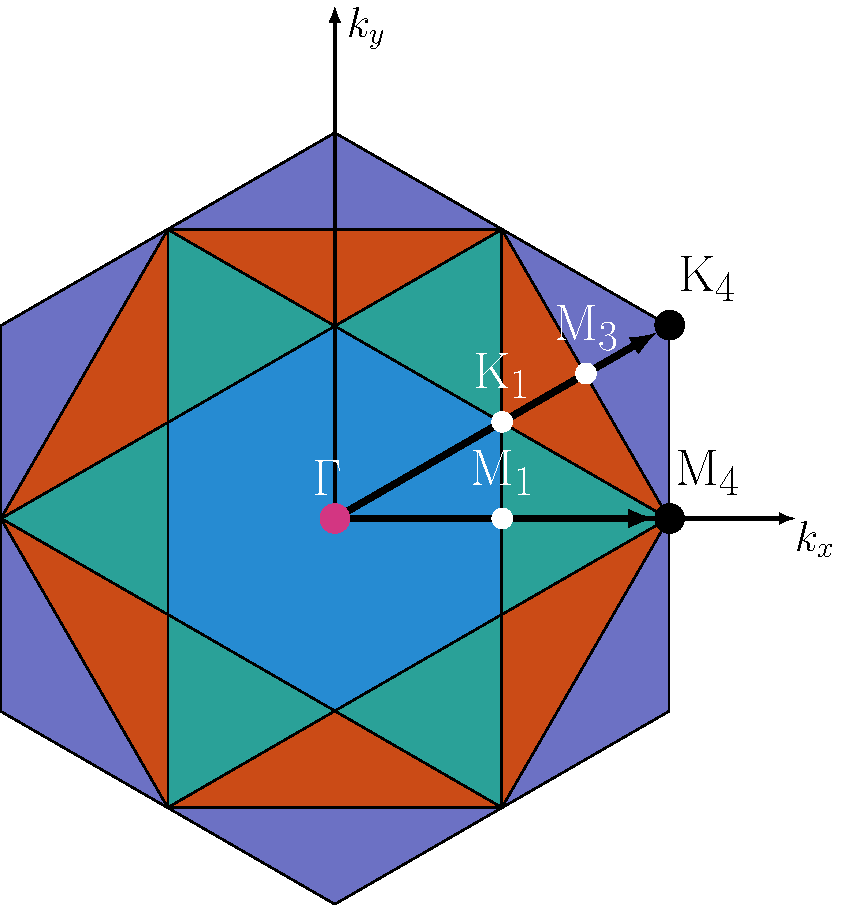
\includegraphics[width=0.6\linewidth]{fig01}
\caption{First four Brillouin zones with the two selected paths
(1) $\Gamma$ to M in the fourth zone (M$_{4}$), and (2) $\Gamma$ to K in the
fourth zone (K$_{4}$), along which we calculate the EEL spectra and macroscopic
dielectric function.}
\label{fig:brillouin}
\end{figure}

Lastly, we used the DP/EXC code \cite{olevanoDP, reiningEXC} to execute the
calculation of the macroscopic dielectric function ($\epsilon$) and the EEL
spectra for different values of $q$. We obtained converged spectra using 12
shells of reciprocal-space vectors ($\mathbf{G}$), 20 shells of plane waves, and
80 total bands for all methods, except when explicitly noted otherwise.
Local-field effects have been taken into account in every calculation presented
here. The macroscopic dielectric functions and EEL spectra have a 0.6\,eV
Gaussian broadening applied to them. Furthermore, in order to simulate the
band-structure stretching, obtained from GW results \cite{olevano}, a
stretching of 10\,\% was applied to the valence-band energies, and 5\,\% to the
conduction band energies. These parameters and corrections were kept uniform
across all methods studied here. 400 iterations were used for calculations that
make use of the Haydock iterative method \cite{haydockJPC72, haydockCPC80,
benedictPRB99, roccaJCP08, gruningCMS11, ljungbergPRB15}.

The DP/EXC code was enabled to use the PETSc \cite{petsc} and SLEPc
\cite{hernandezTOMS05} libraries for diagonalizing \cite{reshetnyakthesis} the
complete excitonic Hamiltonian using MPI parallelism. In fact, it is the
inclusion of these libraries that makes it possible to solve the BSE CP (with
coupling terms included) in a reasonable amount of time. All other calculations
use the OpenMP parallel API, for efficient parallelization and memory use on a
single machine. The Supplemental Materials contain detailed computational
benchmarks concerning these calculations.

%%%%%%%%%%%%%%%%%%%%%%%%%%%%%%%%%%%%%%%%%%%%%%%%%%%%%%%%%%%%%%%%%%%%%%%%%%%%%%%%
%%%%%%%%%%%%%%%%%%%%%%%%%%%%%%%%%%%%%%%%%%%%%%%%%%%%%%%%%%%%%%%%%%%%%%%%%%%%%%%%

\section{Results}\label{sec:results}

We calculate the macroscopic dielectric functions and the subsequent EEL spectra
over an energy range between 0 to 15\,eV, enough to cover the dispersion behavior
of the $\pi$ plasmon for
each value of momentum transfer $q$. Fig. \ref{fig:brillouin} depicts the two
selected in-plane $q$ paths along which we calculate our results. The $\Gamma
\rightarrow \mathrm{M}_{4}$ path has only variation of $q_{x}$, and passes
through the M point of the first zone. The $\Gamma \rightarrow \mathrm{K}_{4}$
path varies both $q_{x}$ and $q_{y}$ and passes through the K point of the first
zone and the M point of the third zone. As mentioned in Sec. \ref{sec:comp}, we
used 14$\times$14$\times$02 and 12$\times$12$\times$02 \textbf{k}-point grids
for these calculations, allowing us to evaluate the $q$-dependence in steps of
1/14 and/or 1/12 for each path. Shared points between these two grids ($\Gamma$,
M$_{1}$, and M$_{4}$) are virtually identical, meaning that both grids have
acceptable convergence.

A plasmon excitation is identified as the point where
$\mathrm{Re}\,\epsilon_{\mathrm{M}} = 0$ (crossing from negative to positive),
and $\mathrm{Im}\,\epsilon_{\mathrm{M}}$ is nearly zero. For convenience, we will
refer to this as the plasmon criterion \cite{jonesbookv11973}; therefore, peaks
in the EEL spectra that meet this condition will naturally be understood to be
plasmon excitations.
The general physical picture of the $q$-dependent plasmon dispersion is as
follows. The shape and intensity of
$\mathrm{Re}\,\epsilon_{\mathrm{M}}(\mathbf{q}, \omega)$ are indicative of the
electron screening behavior, and $\mathrm{Im}\,\epsilon_{\mathrm{M}}(\mathbf{q},
\omega)$ is indicative of interband transitions \cite{marinopoulosPRB04}.
Plasmonic behavior for small values of $q$ are present in the EEL spectrum, with
the thin peaked $\pi$ plasmon appearing around 7\,eV.
For values of $q < 1.0$\,\r{A}$^{-1}$,
the plasmon criterion is met and the plasmon peak occurs very close to the point
where $\mathrm{Re}\,\epsilon_{\mathrm{M}}(\mathbf{q}, \omega)$ is zero. This
holds true for both the $\Gamma \rightarrow \mathrm{M}$, and $\Gamma
\rightarrow \mathrm{K}$ directions. For larger values of $q$, the plasmon
criterion is no longer met, as $\mathrm{Re}\,\epsilon_{\mathrm{M}}(\mathbf{q},
\omega)$ takes on only positive values; however, the EEL spectrum still presents
defined peaks that correspond to interband transitions only
\cite{marinopoulosPRB04}. This is in accordance to Eq. \eqref{eq:eels}, where the
EEL spectra will begin to be less and less affected by the reduced screening of
$\mathrm{Re}\,\epsilon_{\mathrm{M}}(\mathbf{q}, \omega)$, and essentially mimics
$\mathrm{Im}\,\epsilon_{\mathrm{M}}(\mathbf{q}, \omega)$. 

%%%%%%%%%%%%%%%%%%%%%%%%%%%%%%%%%%%%%%%%%%%%%%%%%%%%%%%%%%%%%%%%%%%%%%%%%%%%%%%%

% \subsection{The \texorpdfstring{$\pi$}{pi} Plasmon}

\begin{figure}[t]
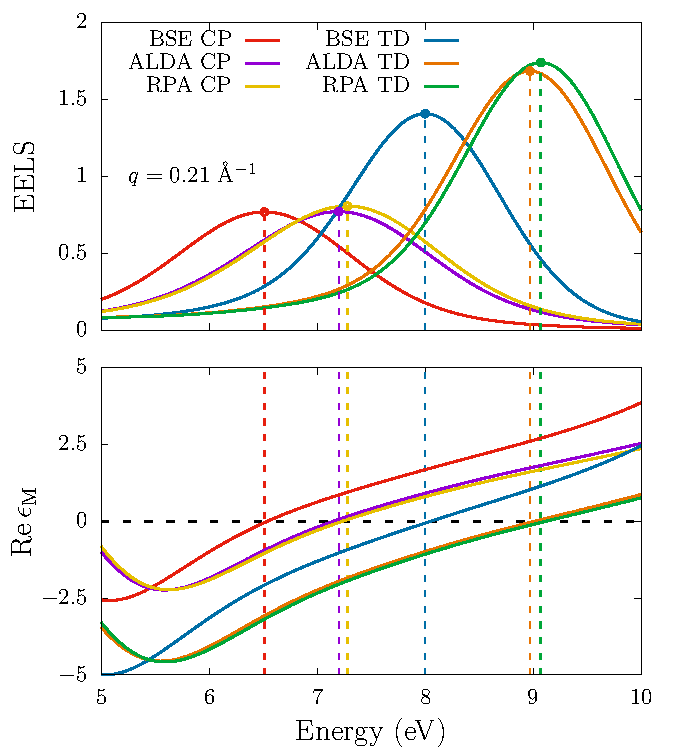
\includegraphics[width=\linewidth]{fig02}
\caption{Top panel:
Comparison of the different theoretical EEL spectra in the $\pi$ plasmon region
at the same momentum transfer $q = 0.21$\,\r{A}$^{-1}$.
Bottom panel: the corresponding real part of the dielectric
function, $\mathrm{Re}\,\epsilon_{\mathrm{M}}$. The plasmon criterion is met for
this low value of $q$; however, the plasmon peak position and intensity varies
widely between each method.}
\label{fig:comparison}
\end{figure}

In Fig. \ref{fig:comparison}, we present a general comparison of the EEL spectra
and macroscopic dielectric function between the different methods, centered
around the energy range of the $\pi$ plasmon. For this low value of $q = 0.21$\,
\r{A}$^{-1}$, the peak in the EEL spectra meets the aforementioned plasmon
criterion and the plasmon peak energy position matches the zero crossing (from
negative to positive) of $\mathrm{Re}\,\epsilon_{\mathrm{M}}(\mathbf{q},
\omega)$. $\mathrm{Im}\,\epsilon_{\mathrm{M}}(\mathbf{q}, \omega)$ (not shown)
is also very small around this transition point. The plasmon peak is present for
all calculated methods; however, peak position and intensity vary significantly
between them. The predominant difference in peak intensity comes from the
inclusion of the coupling terms in the excitonic Hamiltonian.
{\color{red}
Considering the applied broadening, methods that include these coupling terms
(BSE CP, ALDA CP, and RPA CP) have peak intensities that are closer to
experiment \cite{zeppenfeldZP71, buchnerPSSB77, marinopoulosPRB04}; the
remaining methods produce peaks that are roughly twice as intense.
}
The ALDA and RPA calculations yield spectra
that are generally quite similar. We will discuss the peak positions in more
detail below when addressing the $q$-dependent plasmon dispersion.

\begin{figure}[b]
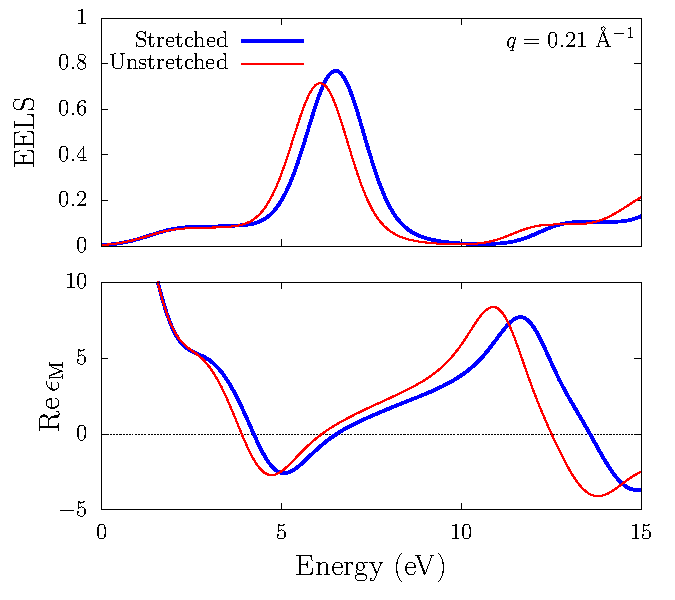
\includegraphics[width=\linewidth]{fig03}
\caption{Top panel: 
EEL spectra calculated with the Bethe-Salpeter equation, including the coupling
terms in the excitonic Hamiltonian (BSE CP), for a transfered momentum
$q = 0.21$\,\r{A}$^{-1}$, calculated with
both stretched and unstretched valence and conduction bands.
Bottom panel: The corresponding real part of the
macrosopic
dielectric function,
$\mathrm{Re}\,\epsilon_{\mathrm{M}}$. The band stretching causes the spectra
peaks to shift non-rigidly to higher energies.}
\label{fig:stretching}
\end{figure}

Fig. \ref{fig:stretching} depicts the differences introduced into both the EEL
spectrum and the dielectric function when applying valence (conduction) band
stretching of 10\% (5\%). As mentioned above, this band stretching is taking
from GW results \cite{olevano} and compare very well with photoemission
measurements \cite{heskePRB99, marinopoulosPRB04}. Both the EEL spectrum and
dielectric function are shifted towards higher energies; however, the nature of
the stretching causes a redistribution of the band energies, which causes
changes in both the peak position and intensities. Since these values are
applied to the DFT band energies that are used subsequently in the calculation
of the dielectric function, this behavior is consistent across all methods, and
for all calculated values of $q$. This stretching improves the
agreement of the peak positions between the calculated and the experimental EELS
spectra.

\begin{figure}[t]
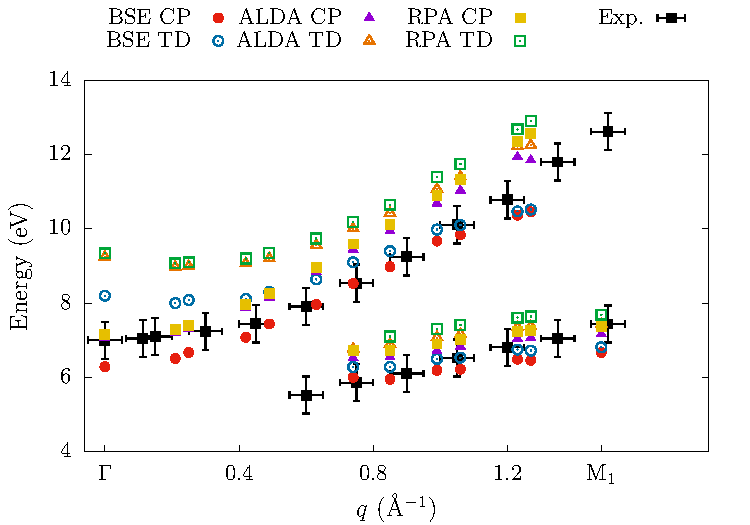
\includegraphics[width=\linewidth]{fig04}
\caption{
The $\pi$ plasmon dispersion, obtained by plotting the peak maximum (in eV) as
a function of transfered momentum $q$ (along the $\Gamma \rightarrow
\mathrm{M}_{1}$ path). The peak positions calculated using each theoretical
method are compared with experimental data from Ref. \onlinecite{liouPRB15}. The
uneven spacing between the calculated points is due to the use of both the
12$\times$12$\times$2 and 14$\times$14$\times$2 \textbf{k}-point grids.
}
\label{fig:gm-dispersion}
\end{figure}

In Fig. \ref{fig:gm-dispersion}, we present the $q$-dependent dispersion
behavior of the $\pi$ plasmon, for values of $q$ along the $\Gamma \rightarrow
\mathrm{M}_{1}$ path. Colored points represent the different calculations, while
the black squares are data points from high-resolution EELS measurements
reproduced with permission from Ref. \onlinecite{liouPRB15}. The peaks in the
EEL spectra split into two branches; a main branch that is present for all
values of $q$ with energy values between 7 and 13\,eV, and a secondary branch
that begins to appear after $q = 0.6$\,\r{A}$^{-1}$ with energy values between 5
and 8\,eV. As mentioned above, not all of these points represent plasmon
excitations; in general, points for values of $q > 1.0$\,\r{A}$^{-1}$ do not meet
the plasmon criterion and are primarily produced by interband transitions
\cite{marinopoulosPRB04}. However, these points are measured by EELS experiments
and are therefore included in our comparison.

It is evident from the plot that the peak positions vary widely across all
methods, and some general trends can be seen. Calculations that employ the TDA
are generally shifted towards higher energies over their counterparts; thus,
ALDA TD and RPA TD typically present the least similarity with the experimental
data. ALDA CP and RPA CP are quite similar, with ALDA CP presenting some
improvement over RPA CP. Both of these methods tend to have a higher energy
value than the experiment, although they fit well for low values of $q$. The BSE
CP calculation coincides well with the experimental points throughout the entire
$q$-range, but tends to underestimate the energy for large values of $q$. Both
BSE calculations begin to coincide as the value of $q$ increases.

In Fig. \ref{fig:gm-dispersion2}, we focus on the upper branch and compare our
most complete calculation, BSE CP, against three separate experimental EELS
measurements taken from Refs. \onlinecite{zeppenfeldZP71},
\onlinecite{kinyanjuiEPL12}, and \onlinecite{liouPRB15}. These experiments are
mostly consistent amongst each other across the range of transfered momentum. Our
calculation yields, in general, quantitatively similar results to the measured
peak values.
All of our calculations follow the well-documented quadratic dispersion relation 
\cite{zeppenfeldZP71, marinopoulosPRB04}; in particular, the BSE CP method
follows this relation for values of $q < 1.2$\,\r{A}$^{-1}$. The red dashed line
in the figure is a quadratic fit for the theoretical points.
Overall, our calculated results can be directly compared with
experiments that span almost five decades, taken by completely different groups.

\begin{figure}[b]
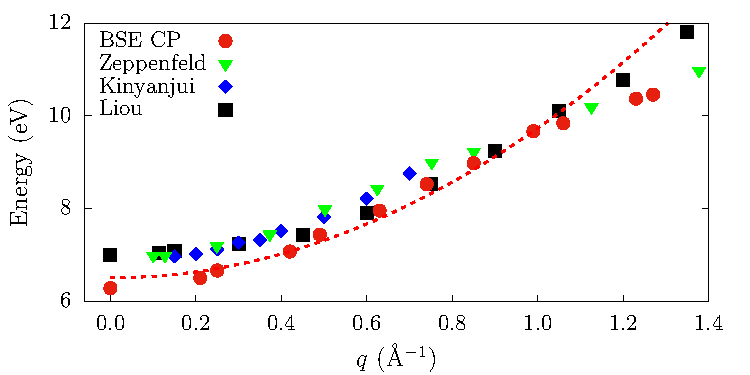
\includegraphics[width=\linewidth]{fig05}
\caption{A more detailed view of the $\pi$ plasmon peak dispersion along the
$\Gamma \rightarrow \mathrm{M}_{1}$ path; ``BSE CP'' is our theoretical result
(featured in Fig. \ref{fig:gm-dispersion}), ``Zeppenfeld'' is experimental data
from Ref. \onlinecite{zeppenfeldZP71}, ``Kinyanjui'' from Ref.
\onlinecite{kinyanjuiEPL12}, and ``Liou'' from Ref. \onlinecite{liouPRB15}.
Errorbars have been excluded from the ``Liou'' data for improved legibility.
The red dashed line is a quadratic fit for the theoretical points.}
\label{fig:gm-dispersion2}
\end{figure}

These trends are in accordance with the approximations implied for each method.
First, taking into account excitons (e-h interactions) causes the peak position
to shift towards lower energies \cite{albrechtPRL98}; second, the inclusion of
the coupling terms in the Hamiltonian further shifts the peak position to lower
energies \cite{olevanoPRL01, gruningNL09}. This explains why BSE CP has the
lowest peak energies, and why RPA TD and ALDA TD have the highest. Furthermore,
the TDA is known to fail at describing plasmonic excitations
\cite{zimmermannPSSB70, caliebePRL00, olevanoPRL01, gruningNL09} due to the
neglected e-h antipairs; thus, for small values of $q$, BSE TD tends to
overestimate the peak energy. However, as the momentum transfer increases the
plasmon dissipates into interband transitions (reducing the number of e-h
antipairs), and the BSE CP and BSE TD calculations begin to coincide. In fact,
this behavior holds true for all methods; in other words, the TDA can accurately
describe the peak positions when plasmon behavior is not expected, or there is
little to no contribution from e-h antipairs.

\begin{figure}[t]
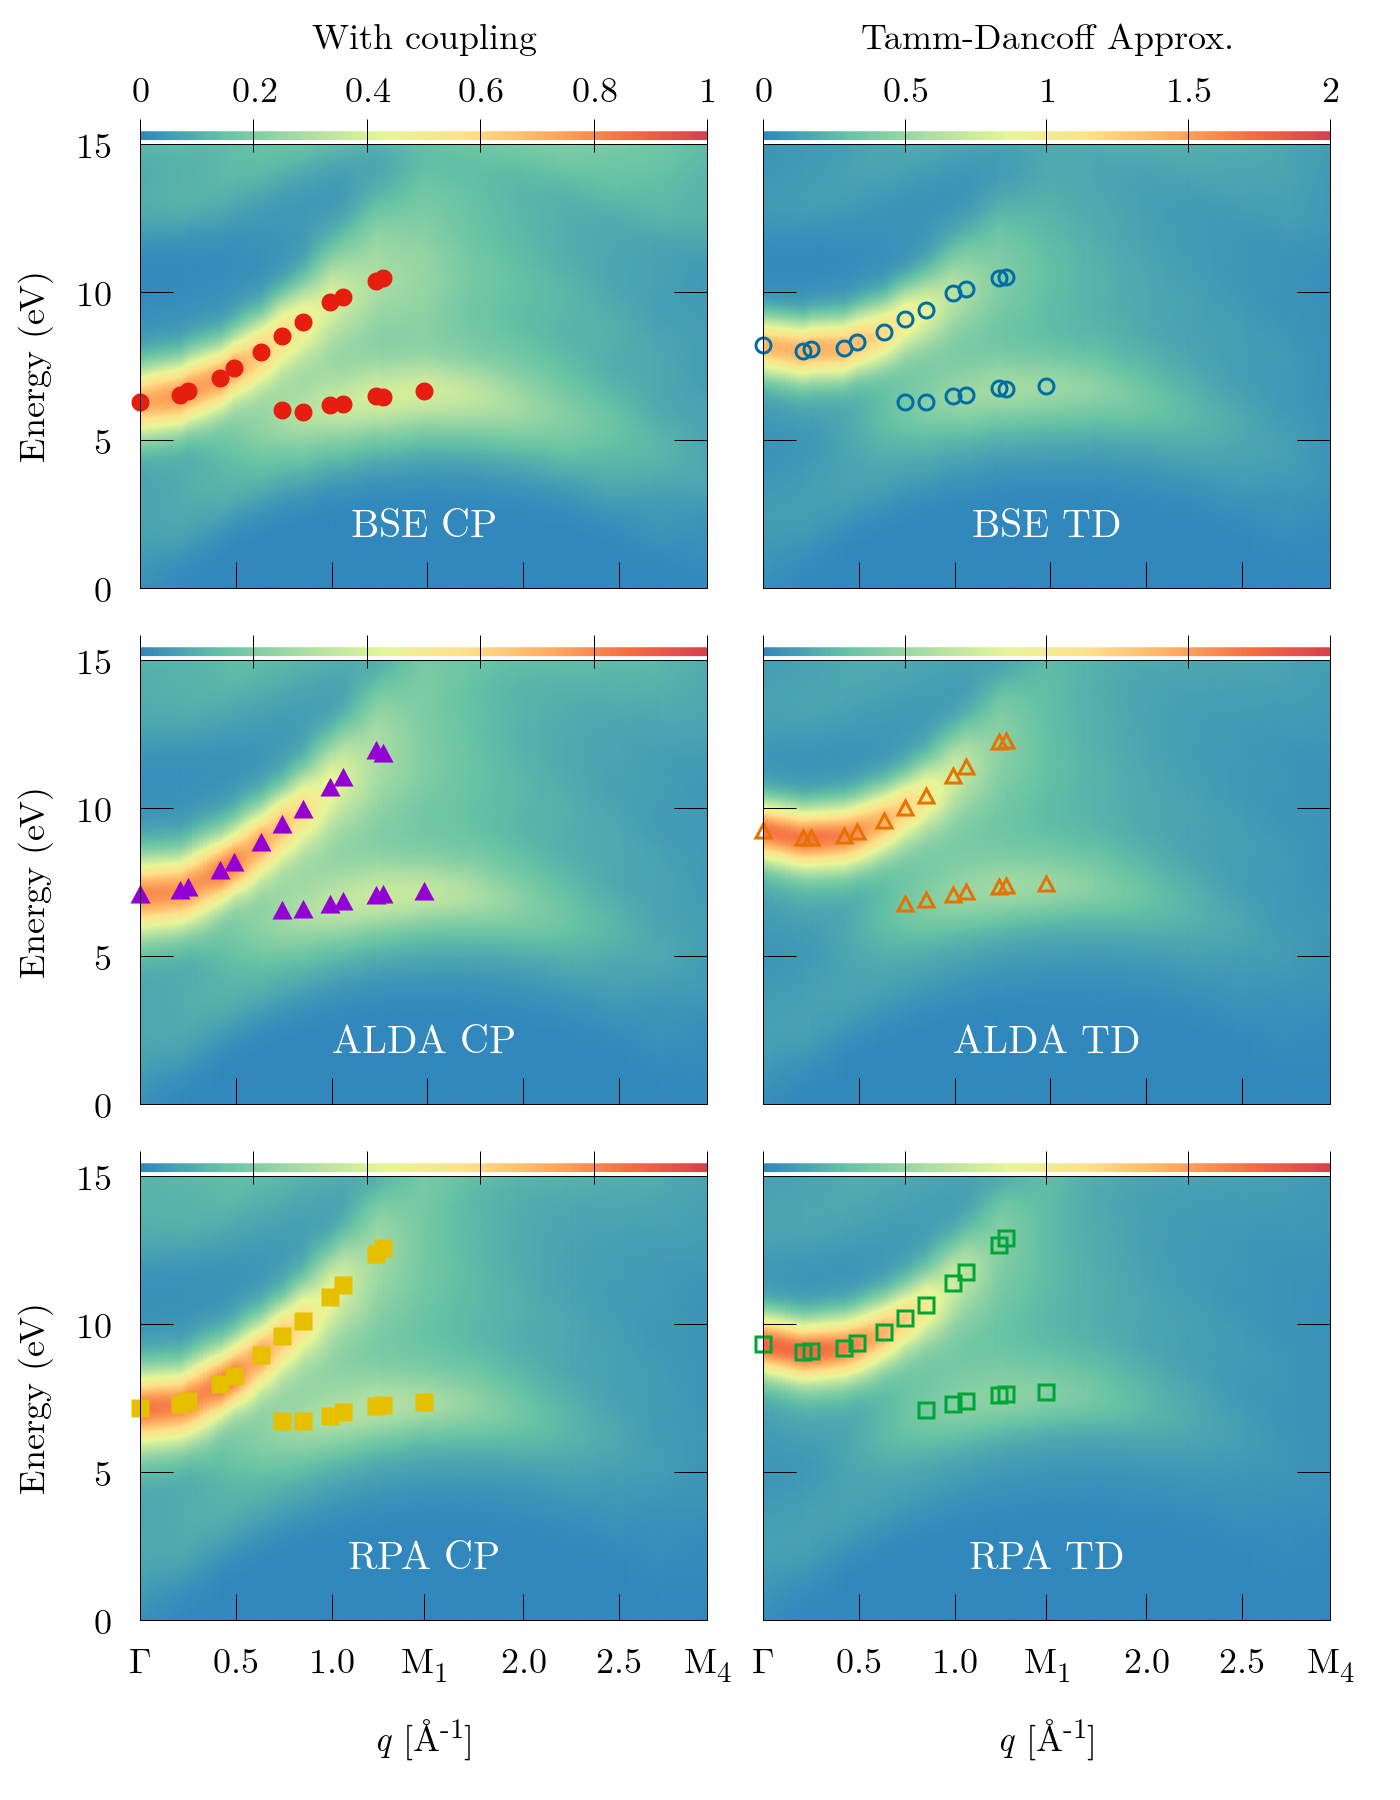
\includegraphics[width=\linewidth]{fig06}
\caption{Color map representations of the calculated EEL spectra vs. transfered momentum
($q$) for the $\pi$ plasmon region, for $q$ values along the $\Gamma \rightarrow
\mathrm{M}_{4}$ path. Methods including the coupling terms in the excitonic
Hamiltonian are shown in the left column, and methods neglecting these terms
(Tamm-Dancoff approximation) are shown in the right column. The EEL intensity is
represented by the color palette ranging from blue to red.
The exact peak positions from Fig. \ref{fig:gm-dispersion} are superimposed on each color
map.}
\label{fig:gm-heatmap_lo}
\end{figure}

In order to elucidate the general trends beyond the experimental data range
(past the M$_{1}$ point in the first Brillouin zone), we extend our calculations
all the way up to the fourth Brillouin zone to the M$_{4}$ point. Fig.
\ref{fig:gm-heatmap_lo} depicts the complete plasmon dispersion for each
calculation, for $q$ values along along the $\Gamma \rightarrow
\mathrm{M}_{4}$ path. The left side of the figure presents the calculated
dispersion including the coupling terms, and the right side with calculations
that neglect them; the EELS intensity scale is located above each column. The
peak positions featured in Fig. \ref{fig:gm-dispersion} are superimposed over
each color map. All methods agree that the upper branch mostly dissipates for
$q$ values beyond M$_{1}$ (1.48\,\r{A}$^{-1}$), whilst the lower branch
continues to exist throughout the range. As mentioned above, the behavior of
both $\epsilon_{1}$ and $\epsilon_{2}$, which does not conform to the plasmon
criterion for these high $q$ values, indicate that these peaks are primarily due
to interband transitions and are not plasmons. Our predictions also show that
the lower branch presents negative dispersion after M$_{1}$, appears to return
to lower energies rather than continuing upwards. Confirmation of this trend
will require future experimental measurements taken at similarly high values of
$q$. While these plots are very useful to discern trends, they show that the
differences between each method are subtle, and must be analyzed in closer
detail as we have in Figs. \ref{fig:gm-dispersion} and \ref{fig:gm-dispersion2}.

\begin{figure}[b]
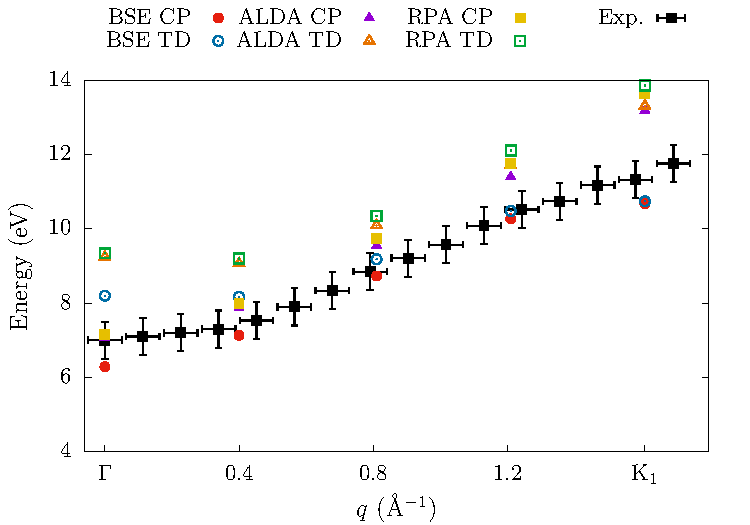
\includegraphics[width=\linewidth]{fig07}
\caption{
The $\pi$ plasmon dispersion, obtained by plotting the peak maximum (in eV) as
a function of transfered momentum $q$ (along the $\Gamma \rightarrow
\mathrm{K}_{1}$ path). The peak positions calculated using each theoretical
method are compared with experimental data from Ref. \onlinecite{liouPRB15}.
}
\label{fig:gk-dispersion}
\end{figure}

Likewise, we conduct a similar analysis for the $\Gamma \rightarrow
\mathrm{K}_{1}$ path in Fig. \ref{fig:gk-dispersion}. For these values of
$q$, the spectra is dominated by a single peak with energy positions ranging
from 7 to 12\,eV, where the classical plasmonic behavior is lost after $q\approx
1.00$\,\r{A}$^{-1}$. Once again, our calculations confirm the strong dispersion
of the peak position. ALDA TD and RPA TD significantly overestimate the peak
energy position, and CP and TD calculations begin to coincide for increasing
momentum transfer. BSE calculations yield good agreement with experiment
throughout the range. We also extend our calculations for increasing $q$ values
into the fourth Brillouin zone K$_{4}$ point.

The Supplemental Material \cite{supplement} features a similar analysis of the $\pi + \sigma$
plasmon that occurs in the 25--45\,eV energy range. We review the trends of each
theoretical method, as there is little experimental data available for this
energy range.

%%%%%%%%%%%%%%%%%%%%%%%%%%%%%%%%%%%%%%%%%%%%%%%%%%%%%%%%%%%%%%%%%%%%%%%%%%%%%%%%
%%%%%%%%%%%%%%%%%%%%%%%%%%%%%%%%%%%%%%%%%%%%%%%%%%%%%%%%%%%%%%%%%%%%%%%%%%%%%%%%

\section{Conclusions}\label{sec:conclusions}

We carried out a systematic study of the macroscopic dielectric function and EEL
spectra for the $\pi$ plasmon of graphite, comparing \emph{ab initio} TDDFT and
BSE methods. We selected graphite as a good benchmark case due to the extensive
theoretical and experimental work available. Our results coincide with previous
literature (where available), and offer quantitative agreement with experiment.
Using two non-equivalent momentum paths spanning the first four Brillouin zones,
we demonstrate the importance of including the coupling terms in the excitonic
Hamiltonian for describing plasmon excitations. The TDA, while numerically
efficient, cannot reproduce some key features in the experimental EEL spectra.
Access to high-resolution EELS measurements around the $\pi$ plasmon allow us to
compare the detailed behavior and trends of each method.

Overall, we provide an overview of \emph{ab initio} methods that are considered
state-of-the-art at describing the optoelectronic properties of solid state
systems. We have applied these methods on graphite, which offers an excellent
benchmark material for this type of study. We are confident this study can be
used as reference for future work. The knowledge of the inverse dielectric
function for the wide range of momentum transfer (beyond the
experimental range available today) that we provide, gives useful insights also
for other methods which are intrinsically based on the concept of Coulomb
screening, like many-body GW (and beyond GW) approaches \cite{rodlPRB17,
luciabook}, hybrid functionals in DFT \cite{krukauJCP06}, or Dynamical Mean
Field Theory \cite{biermannJPCM14}.

Finally, we present real-world computational benchmarks in the Supplemental
Materials \cite{supplement}; as these clearly show, the significant computational cost of BSE CP
may not be necessarily warranted for every situation. The very low computational
expense of the TDDFT methods compared to the BSE, make them an attractive
alternative when the coupling terms are the determining factors for a
calculation. In summary, these methods should always be applied judiciously and
their use evaluated on a case by case basis.

%%%%%%%%%%%%%%%%%%%%%%%%%%%%%%%%%%%%%%%%%%%%%%%%%%%%%%%%%%%%%%%%%%%%%%%%%%%%%%%%
%%%%%%%%%%%%%%%%%%%%%%%%%%%%%%%%%%%%%%%%%%%%%%%%%%%%%%%%%%%%%%%%%%%%%%%%%%%%%%%%

\section{Acknowledgments}

The authors would like to thank S. C. Liou for graciously contributing the
experimental data featured in this work, and also M. Gatti and I. Reshetnyak for
fruitful discussion. The authors thankfully acknowledge the computer resources,
technical expertise, and support provided by the Laboratorio Nacional de
Superc\'omputo del Sureste de M\'exico, a member of the CONACYT network of
national laboratories. S. M. Anderson acknowledges partial support for this
project from CONACYT-M\'exico scholarship 349278. B. S. Mendoza acknowledges
funding from CONACYT-Mexico research project A1-S-9410.

%%%%%%%%%%%%%%%%%%%%%%%%%%%%%%%%%%%%%%%%%%%%%%%%%%%%%%%%%%%%%%%%%%%%%%%%%%%%%%%%
%%%%%%%%%%%%%%%%%%%%%%%%%%%%%%%%%%%%%%%%%%%%%%%%%%%%%%%%%%%%%%%%%%%%%%%%%%%%%%%%

%merlin.mbs apsrev4-1.bst 2010-07-25 4.21a (PWD, AO, DPC) hacked
%Control: key (0)
%Control: author (72) initials jnrlst
%Control: editor formatted (1) identically to author
%Control: production of article title (-1) disabled
%Control: page (0) single
%Control: year (1) truncated
%Control: production of eprint (0) enabled
\begin{thebibliography}{77}%
\makeatletter
\providecommand \@ifxundefined [1]{%
 \@ifx{#1\undefined}
}%
\providecommand \@ifnum [1]{%
 \ifnum #1\expandafter \@firstoftwo
 \else \expandafter \@secondoftwo
 \fi
}%
\providecommand \@ifx [1]{%
 \ifx #1\expandafter \@firstoftwo
 \else \expandafter \@secondoftwo
 \fi
}%
\providecommand \natexlab [1]{#1}%
\providecommand \enquote  [1]{``#1''}%
\providecommand \bibnamefont  [1]{#1}%
\providecommand \bibfnamefont [1]{#1}%
\providecommand \citenamefont [1]{#1}%
\providecommand \href@noop [0]{\@secondoftwo}%
\providecommand \href [0]{\begingroup \@sanitize@url \@href}%
\providecommand \@href[1]{\@@startlink{#1}\@@href}%
\providecommand \@@href[1]{\endgroup#1\@@endlink}%
\providecommand \@sanitize@url [0]{\catcode `\\12\catcode `\$12\catcode
  `\&12\catcode `\#12\catcode `\^12\catcode `\_12\catcode `\%12\relax}%
\providecommand \@@startlink[1]{}%
\providecommand \@@endlink[0]{}%
\providecommand \url  [0]{\begingroup\@sanitize@url \@url }%
\providecommand \@url [1]{\endgroup\@href {#1}{\urlprefix }}%
\providecommand \urlprefix  [0]{URL }%
\providecommand \Eprint [0]{\href }%
\providecommand \doibase [0]{http://dx.doi.org/}%
\providecommand \selectlanguage [0]{\@gobble}%
\providecommand \bibinfo  [0]{\@secondoftwo}%
\providecommand \bibfield  [0]{\@secondoftwo}%
\providecommand \translation [1]{[#1]}%
\providecommand \BibitemOpen [0]{}%
\providecommand \bibitemStop [0]{}%
\providecommand \bibitemNoStop [0]{.\EOS\space}%
\providecommand \EOS [0]{\spacefactor3000\relax}%
\providecommand \BibitemShut  [1]{\csname bibitem#1\endcsname}%
\let\auto@bib@innerbib\@empty
%</preamble>
\bibitem [{\citenamefont {Hohenberg}\ and\ \citenamefont
  {Kohn}(1964)}]{hohenbergPR64}%
  \BibitemOpen
  \bibfield  {author} {\bibinfo {author} {\bibfnamefont {P.}~\bibnamefont
  {Hohenberg}}\ and\ \bibinfo {author} {\bibfnamefont {W.}~\bibnamefont
  {Kohn}},\ }\href {http://link.aps.org/doi/10.1103/PhysRev.136.B864}
  {\bibfield  {journal} {\bibinfo  {journal} {Phys. Rev.}\ }\textbf {\bibinfo
  {volume} {136}},\ \bibinfo {pages} {B864} (\bibinfo {year}
  {1964})}\BibitemShut {NoStop}%
\bibitem [{\citenamefont {Kohn}\ and\ \citenamefont {Sham}(1965)}]{kohnPR65}%
  \BibitemOpen
  \bibfield  {author} {\bibinfo {author} {\bibfnamefont {W.}~\bibnamefont
  {Kohn}}\ and\ \bibinfo {author} {\bibfnamefont {L.~J.}\ \bibnamefont
  {Sham}},\ }\href {\doibase 10.1103/PhysRev.140.A1133} {\bibfield  {journal}
  {\bibinfo  {journal} {Phys. Rev.}\ }\textbf {\bibinfo {volume} {140}},\
  \bibinfo {pages} {A1133} (\bibinfo {year} {1965})}\BibitemShut {NoStop}%
\bibitem [{\citenamefont {Runge}\ and\ \citenamefont
  {Gross}(1984)}]{rungePRL84}%
  \BibitemOpen
  \bibfield  {author} {\bibinfo {author} {\bibfnamefont {E.}~\bibnamefont
  {Runge}}\ and\ \bibinfo {author} {\bibfnamefont {E.~K.~U.}\ \bibnamefont
  {Gross}},\ }\href {\doibase 10.1103/PhysRevLett.52.997} {\bibfield  {journal}
  {\bibinfo  {journal} {Phys. Rev. Lett.}\ }\textbf {\bibinfo {volume} {52}},\
  \bibinfo {pages} {997} (\bibinfo {year} {1984})}\BibitemShut {NoStop}%
\bibitem [{\citenamefont {Onida}\ \emph {et~al.}(2002)\citenamefont {Onida},
  \citenamefont {Reining},\ and\ \citenamefont {Rubio}}]{onidaRMP02}%
  \BibitemOpen
  \bibfield  {author} {\bibinfo {author} {\bibfnamefont {G.}~\bibnamefont
  {Onida}}, \bibinfo {author} {\bibfnamefont {L.}~\bibnamefont {Reining}}, \
  and\ \bibinfo {author} {\bibfnamefont {A.}~\bibnamefont {Rubio}},\ }\href
  {\doibase 10.1103/RevModPhys.74.601} {\bibfield  {journal} {\bibinfo
  {journal} {Rev. Mod. Phys.}\ }\textbf {\bibinfo {volume} {74}},\ \bibinfo
  {pages} {601} (\bibinfo {year} {2002})}\BibitemShut {NoStop}%
\bibitem [{\citenamefont {Gavrilenko}\ and\ \citenamefont
  {Bechstedt}(1997)}]{gavrilenkoPRB97}%
  \BibitemOpen
  \bibfield  {author} {\bibinfo {author} {\bibfnamefont {V.~I.}\ \bibnamefont
  {Gavrilenko}}\ and\ \bibinfo {author} {\bibfnamefont {F.}~\bibnamefont
  {Bechstedt}},\ }\href {\doibase 10.1103/PhysRevB.55.4343} {\bibfield
  {journal} {\bibinfo  {journal} {Phys. Rev. B}\ }\textbf {\bibinfo {volume}
  {55}},\ \bibinfo {pages} {4343} (\bibinfo {year} {1997})}\BibitemShut
  {NoStop}%
\bibitem [{\citenamefont {Fetter}\ and\ \citenamefont
  {Walecka}(1972)}]{fetterbook72}%
  \BibitemOpen
  \bibfield  {author} {\bibinfo {author} {\bibfnamefont {A.~L.}\ \bibnamefont
  {Fetter}}\ and\ \bibinfo {author} {\bibfnamefont {J.~D.}\ \bibnamefont
  {Walecka}},\ }\href {http://physicstoday.scitation.org/doi/10.1063/1.3071096}
  {\emph {\bibinfo {title} {Quantum {Theory} of {Many} {Particle}
  {Systems}}}},\ Vol.~\bibinfo {volume} {25}\ (\bibinfo  {publisher}
  {McGraw-Hill, Inc.},\ \bibinfo {year} {1972})\BibitemShut {NoStop}%
\bibitem [{\citenamefont {Hedin}(1965)}]{hedinPR65}%
  \BibitemOpen
  \bibfield  {author} {\bibinfo {author} {\bibfnamefont {L.}~\bibnamefont
  {Hedin}},\ }\href {http://link.aps.org/doi/10.1103/PhysRev.139.A796}
  {\bibfield  {journal} {\bibinfo  {journal} {Phys. Rev.}\ }\textbf {\bibinfo
  {volume} {139}},\ \bibinfo {pages} {A796} (\bibinfo {year}
  {1965})}\BibitemShut {NoStop}%
\bibitem [{\citenamefont {Salpeter}\ and\ \citenamefont
  {Bethe}(1951)}]{salpeterPR51}%
  \BibitemOpen
  \bibfield  {author} {\bibinfo {author} {\bibfnamefont {E.~E.}\ \bibnamefont
  {Salpeter}}\ and\ \bibinfo {author} {\bibfnamefont {H.~A.}\ \bibnamefont
  {Bethe}},\ }\href {http://prola.aps.org/abstract/PR/v84/i6/p1232_1}
  {\bibfield  {journal} {\bibinfo  {journal} {Phys. Rev.}\ }\textbf {\bibinfo
  {volume} {84}},\ \bibinfo {pages} {1232} (\bibinfo {year}
  {1951})}\BibitemShut {NoStop}%
\bibitem [{\citenamefont {Abrikosov}\ \emph {et~al.}(1965)\citenamefont
  {Abrikosov}, \citenamefont {Gorlcov},\ and\ \citenamefont
  {Illyaloslinski}}]{abrikosovbook65}%
  \BibitemOpen
  \bibfield  {author} {\bibinfo {author} {\bibfnamefont {A.~A.}\ \bibnamefont
  {Abrikosov}}, \bibinfo {author} {\bibfnamefont {L.~P.}\ \bibnamefont
  {Gorlcov}}, \ and\ \bibinfo {author} {\bibfnamefont {I.~E.}\ \bibnamefont
  {Illyaloslinski}},\ }\href@noop {} {\emph {\bibinfo {title} {Methods of
  {Quantum} {Field} {Theory} in {Statistical} {Physics}}}},\ \bibinfo {series}
  {Quantum {Field} {Theoretical} {Methods} in {Statistical} {Physics}},
  Vol.~\bibinfo {volume} {4}\ (\bibinfo  {publisher} {Pergamon Press},\
  \bibinfo {year} {1965})\BibitemShut {NoStop}%
\bibitem [{\citenamefont {Sham}\ and\ \citenamefont {Rice}(1966)}]{shamPR66}%
  \BibitemOpen
  \bibfield  {author} {\bibinfo {author} {\bibfnamefont {L.~J.}\ \bibnamefont
  {Sham}}\ and\ \bibinfo {author} {\bibfnamefont {T.~M.}\ \bibnamefont
  {Rice}},\ }\href {\doibase 10.1103/PhysRev.144.708} {\bibfield  {journal}
  {\bibinfo  {journal} {Phys. Rev.}\ }\textbf {\bibinfo {volume} {144}},\
  \bibinfo {pages} {708} (\bibinfo {year} {1966})}\BibitemShut {NoStop}%
\bibitem [{\citenamefont {Hanke}\ and\ \citenamefont
  {Sham}(1980)}]{hankePRB80}%
  \BibitemOpen
  \bibfield  {author} {\bibinfo {author} {\bibfnamefont {W.}~\bibnamefont
  {Hanke}}\ and\ \bibinfo {author} {\bibfnamefont {L.~J.}\ \bibnamefont
  {Sham}},\ }\href {http://journals.aps.org/prb/abstract/10.1103/
  PhysRevB.21.4656} {\bibfield  {journal} {\bibinfo  {journal} {Phys. Rev. B}\
  }\textbf {\bibinfo {volume} {21}},\ \bibinfo {pages} {4656} (\bibinfo {year}
  {1980})}\BibitemShut {NoStop}%
\bibitem [{\citenamefont {Shirley}\ and\ \citenamefont
  {Louie}(1993)}]{shirleyPRL93}%
  \BibitemOpen
  \bibfield  {author} {\bibinfo {author} {\bibfnamefont {E.~L.}\ \bibnamefont
  {Shirley}}\ and\ \bibinfo {author} {\bibfnamefont {S.~G.}\ \bibnamefont
  {Louie}},\ }\href {\doibase 10.1103/PhysRevLett.71.133} {\bibfield  {journal}
  {\bibinfo  {journal} {Phys. Rev. Lett.}\ }\textbf {\bibinfo {volume} {71}},\
  \bibinfo {pages} {133} (\bibinfo {year} {1993})}\BibitemShut {NoStop}%
\bibitem [{\citenamefont {Albrecht}\ \emph {et~al.}(1997)\citenamefont
  {Albrecht}, \citenamefont {Onida},\ and\ \citenamefont
  {Reining}}]{albrechtPRB97}%
  \BibitemOpen
  \bibfield  {author} {\bibinfo {author} {\bibfnamefont {S.}~\bibnamefont
  {Albrecht}}, \bibinfo {author} {\bibfnamefont {G.}~\bibnamefont {Onida}}, \
  and\ \bibinfo {author} {\bibfnamefont {L.}~\bibnamefont {Reining}},\ }\href
  {\doibase 10.1103/PhysRevB.55.10278} {\bibfield  {journal} {\bibinfo
  {journal} {Phys. Rev. B}\ }\textbf {\bibinfo {volume} {55}},\ \bibinfo
  {pages} {10278} (\bibinfo {year} {1997})}\BibitemShut {NoStop}%
\bibitem [{\citenamefont {Benedict}\ \emph
  {et~al.}(1998{\natexlab{a}})\citenamefont {Benedict}, \citenamefont
  {Shirley},\ and\ \citenamefont {Bohn}}]{benedictPRL98}%
  \BibitemOpen
  \bibfield  {author} {\bibinfo {author} {\bibfnamefont {L.~X.}\ \bibnamefont
  {Benedict}}, \bibinfo {author} {\bibfnamefont {E.~L.}\ \bibnamefont
  {Shirley}}, \ and\ \bibinfo {author} {\bibfnamefont {R.~B.}\ \bibnamefont
  {Bohn}},\ }\href {\doibase 10.1103/PhysRevLett.80.4514} {\bibfield  {journal}
  {\bibinfo  {journal} {Phys. Rev. Lett.}\ }\textbf {\bibinfo {volume} {80}},\
  \bibinfo {pages} {4514} (\bibinfo {year} {1998}{\natexlab{a}})}\BibitemShut
  {NoStop}%
\bibitem [{\citenamefont {Benedict}\ and\ \citenamefont
  {Shirley}(1999)}]{benedictPRB99}%
  \BibitemOpen
  \bibfield  {author} {\bibinfo {author} {\bibfnamefont {L.~X.}\ \bibnamefont
  {Benedict}}\ and\ \bibinfo {author} {\bibfnamefont {E.~L.}\ \bibnamefont
  {Shirley}},\ }\href {\doibase 10.1103/PhysRevB.59.5441} {\bibfield  {journal}
  {\bibinfo  {journal} {Phys. Rev. B}\ }\textbf {\bibinfo {volume} {59}},\
  \bibinfo {pages} {5441} (\bibinfo {year} {1999})}\BibitemShut {NoStop}%
\bibitem [{\citenamefont {Benedict}\ \emph {et~al.}(2003)\citenamefont
  {Benedict}, \citenamefont {Puzder}, \citenamefont {Williamson}, \citenamefont
  {Grossman}, \citenamefont {Galli}, \citenamefont {Klepeis}, \citenamefont
  {Raty},\ and\ \citenamefont {Pankratov}}]{benedictPRB03}%
  \BibitemOpen
  \bibfield  {author} {\bibinfo {author} {\bibfnamefont {L.~X.}\ \bibnamefont
  {Benedict}}, \bibinfo {author} {\bibfnamefont {A.}~\bibnamefont {Puzder}},
  \bibinfo {author} {\bibfnamefont {A.~J.}\ \bibnamefont {Williamson}},
  \bibinfo {author} {\bibfnamefont {J.~C.}\ \bibnamefont {Grossman}}, \bibinfo
  {author} {\bibfnamefont {G.}~\bibnamefont {Galli}}, \bibinfo {author}
  {\bibfnamefont {J.~E.}\ \bibnamefont {Klepeis}}, \bibinfo {author}
  {\bibfnamefont {J.-Y.}\ \bibnamefont {Raty}}, \ and\ \bibinfo {author}
  {\bibfnamefont {O.}~\bibnamefont {Pankratov}},\ }\href {\doibase
  10.1103/PhysRevB.68.085310} {\bibfield  {journal} {\bibinfo  {journal} {Phys.
  Rev. B}\ }\textbf {\bibinfo {volume} {68}},\ \bibinfo {pages} {085310}
  (\bibinfo {year} {2003})}\BibitemShut {NoStop}%
\bibitem [{\citenamefont {Palummo}\ \emph {et~al.}(2004)\citenamefont
  {Palummo}, \citenamefont {Pulci}, \citenamefont {Del~Sole}, \citenamefont
  {Marini}, \citenamefont {Hahn}, \citenamefont {Schmidt},\ and\ \citenamefont
  {Bechstedt}}]{palummoJPCM04}%
  \BibitemOpen
  \bibfield  {author} {\bibinfo {author} {\bibfnamefont {M.}~\bibnamefont
  {Palummo}}, \bibinfo {author} {\bibfnamefont {O.}~\bibnamefont {Pulci}},
  \bibinfo {author} {\bibfnamefont {R.}~\bibnamefont {Del~Sole}}, \bibinfo
  {author} {\bibfnamefont {A.}~\bibnamefont {Marini}}, \bibinfo {author}
  {\bibfnamefont {P.}~\bibnamefont {Hahn}}, \bibinfo {author} {\bibfnamefont
  {W.~G.}\ \bibnamefont {Schmidt}}, \ and\ \bibinfo {author} {\bibfnamefont
  {F.}~\bibnamefont {Bechstedt}},\ }\href {\doibase
  10.1088/0953-8984/16/39/006} {\bibfield  {journal} {\bibinfo  {journal} {J.
  Phys. Condens. Matter}\ }\textbf {\bibinfo {volume} {16}},\ \bibinfo {pages}
  {S4313} (\bibinfo {year} {2004})}\BibitemShut {NoStop}%
\bibitem [{\citenamefont {Sitt}\ \emph {et~al.}(2007)\citenamefont {Sitt},
  \citenamefont {Kronik}, \citenamefont {Ismail-Beigi},\ and\ \citenamefont
  {Chelikowsky}}]{sittPRA07}%
  \BibitemOpen
  \bibfield  {author} {\bibinfo {author} {\bibfnamefont {A.}~\bibnamefont
  {Sitt}}, \bibinfo {author} {\bibfnamefont {L.}~\bibnamefont {Kronik}},
  \bibinfo {author} {\bibfnamefont {S.}~\bibnamefont {Ismail-Beigi}}, \ and\
  \bibinfo {author} {\bibfnamefont {J.~R.}\ \bibnamefont {Chelikowsky}},\
  }\href {\doibase 10.1103/PhysRevA.76.054501} {\bibfield  {journal} {\bibinfo
  {journal} {Phys. Rev. A}\ }\textbf {\bibinfo {volume} {76}},\ \bibinfo
  {pages} {054501} (\bibinfo {year} {2007})}\BibitemShut {NoStop}%
\bibitem [{\citenamefont {Ramos}\ \emph {et~al.}(2008)\citenamefont {Ramos},
  \citenamefont {Paier}, \citenamefont {Kresse},\ and\ \citenamefont
  {Bechstedt}}]{ramosPRB08}%
  \BibitemOpen
  \bibfield  {author} {\bibinfo {author} {\bibfnamefont {L.~E.}\ \bibnamefont
  {Ramos}}, \bibinfo {author} {\bibfnamefont {J.}~\bibnamefont {Paier}},
  \bibinfo {author} {\bibfnamefont {G.}~\bibnamefont {Kresse}}, \ and\ \bibinfo
  {author} {\bibfnamefont {F.}~\bibnamefont {Bechstedt}},\ }\href {\doibase
  10.1103/PhysRevB.78.195423} {\bibfield  {journal} {\bibinfo  {journal} {Phys.
  Rev. B}\ }\textbf {\bibinfo {volume} {78}},\ \bibinfo {pages} {195423}
  (\bibinfo {year} {2008})}\BibitemShut {NoStop}%
\bibitem [{\citenamefont {Rocca}\ \emph {et~al.}(2010)\citenamefont {Rocca},
  \citenamefont {Lu},\ and\ \citenamefont {Galli}}]{roccaJCP10}%
  \BibitemOpen
  \bibfield  {author} {\bibinfo {author} {\bibfnamefont {D.}~\bibnamefont
  {Rocca}}, \bibinfo {author} {\bibfnamefont {D.}~\bibnamefont {Lu}}, \ and\
  \bibinfo {author} {\bibfnamefont {G.}~\bibnamefont {Galli}},\ }\href
  {\doibase 10.1063/1.3494540} {\bibfield  {journal} {\bibinfo  {journal} {J.
  Chem. Phys.}\ }\textbf {\bibinfo {volume} {133}},\ \bibinfo {pages} {164109}
  (\bibinfo {year} {2010})}\BibitemShut {NoStop}%
\bibitem [{\citenamefont {Garcia-Lastra}\ \emph {et~al.}(2011)\citenamefont
  {Garcia-Lastra}, \citenamefont {Bass},\ and\ \citenamefont
  {Thygesen}}]{garciaJCP11}%
  \BibitemOpen
  \bibfield  {author} {\bibinfo {author} {\bibfnamefont {J.~M.}\ \bibnamefont
  {Garcia-Lastra}}, \bibinfo {author} {\bibfnamefont {J.~D.}\ \bibnamefont
  {Bass}}, \ and\ \bibinfo {author} {\bibfnamefont {K.~S.}\ \bibnamefont
  {Thygesen}},\ }\href {\doibase 10.1063/1.3645544} {\bibfield  {journal}
  {\bibinfo  {journal} {J. Chem. Phys.}\ }\textbf {\bibinfo {volume} {135}},\
  \bibinfo {pages} {121101} (\bibinfo {year} {2011})}\BibitemShut {NoStop}%
\bibitem [{\citenamefont {Gr{\"u}ning}\ \emph {et~al.}(2011)\citenamefont
  {Gr{\"u}ning}, \citenamefont {Marini},\ and\ \citenamefont
  {Gonze}}]{gruningCMS11}%
  \BibitemOpen
  \bibfield  {author} {\bibinfo {author} {\bibfnamefont {M.}~\bibnamefont
  {Gr{\"u}ning}}, \bibinfo {author} {\bibfnamefont {A.}~\bibnamefont {Marini}},
  \ and\ \bibinfo {author} {\bibfnamefont {X.}~\bibnamefont {Gonze}},\ }\href
  {\doibase 10.1016/j.commatsci.2011.02.021} {\bibfield  {journal} {\bibinfo
  {journal} {Comput. Mater. Sci}\ }\textbf {\bibinfo {volume} {50}},\ \bibinfo
  {pages} {2148} (\bibinfo {year} {2011})}\BibitemShut {NoStop}%
\bibitem [{\citenamefont {Gatti}\ and\ \citenamefont
  {Sottile}(2013)}]{gattiPRB13}%
  \BibitemOpen
  \bibfield  {author} {\bibinfo {author} {\bibfnamefont {M.}~\bibnamefont
  {Gatti}}\ and\ \bibinfo {author} {\bibfnamefont {F.}~\bibnamefont
  {Sottile}},\ }\href {\doibase 10.1103/PhysRevB.88.155113} {\bibfield
  {journal} {\bibinfo  {journal} {Phys. Rev. B}\ }\textbf {\bibinfo {volume}
  {88}},\ \bibinfo {pages} {155113} (\bibinfo {year} {2013})}\BibitemShut
  {NoStop}%
\bibitem [{\citenamefont {Onida}\ \emph {et~al.}(1995)\citenamefont {Onida},
  \citenamefont {Reining}, \citenamefont {Godby}, \citenamefont {Del~Sole},\
  and\ \citenamefont {Andreoni}}]{onidaPRL95}%
  \BibitemOpen
  \bibfield  {author} {\bibinfo {author} {\bibfnamefont {G.}~\bibnamefont
  {Onida}}, \bibinfo {author} {\bibfnamefont {L.}~\bibnamefont {Reining}},
  \bibinfo {author} {\bibfnamefont {R.~W.}\ \bibnamefont {Godby}}, \bibinfo
  {author} {\bibfnamefont {R.}~\bibnamefont {Del~Sole}}, \ and\ \bibinfo
  {author} {\bibfnamefont {W.}~\bibnamefont {Andreoni}},\ }\href {\doibase
  10.1103/PhysRevLett.75.818} {\bibfield  {journal} {\bibinfo  {journal} {Phys.
  Rev. Lett.}\ }\textbf {\bibinfo {volume} {75}},\ \bibinfo {pages} {818}
  (\bibinfo {year} {1995})}\BibitemShut {NoStop}%
\bibitem [{\citenamefont {Albrecht}\ \emph {et~al.}(1998)\citenamefont
  {Albrecht}, \citenamefont {Reining}, \citenamefont {Del~Sole},\ and\
  \citenamefont {Onida}}]{albrechtPRL98}%
  \BibitemOpen
  \bibfield  {author} {\bibinfo {author} {\bibfnamefont {S.}~\bibnamefont
  {Albrecht}}, \bibinfo {author} {\bibfnamefont {L.}~\bibnamefont {Reining}},
  \bibinfo {author} {\bibfnamefont {R.}~\bibnamefont {Del~Sole}}, \ and\
  \bibinfo {author} {\bibfnamefont {G.}~\bibnamefont {Onida}},\ }\href
  {\doibase 10.1103/PhysRevLett.80.4510} {\bibfield  {journal} {\bibinfo
  {journal} {Phys. Rev. Lett.}\ }\textbf {\bibinfo {volume} {80}},\ \bibinfo
  {pages} {4510} (\bibinfo {year} {1998})}\BibitemShut {NoStop}%
\bibitem [{\citenamefont {Benedict}\ \emph
  {et~al.}(1998{\natexlab{b}})\citenamefont {Benedict}, \citenamefont
  {Shirley},\ and\ \citenamefont {Bohn}}]{benedictPRB98}%
  \BibitemOpen
  \bibfield  {author} {\bibinfo {author} {\bibfnamefont {L.~X.}\ \bibnamefont
  {Benedict}}, \bibinfo {author} {\bibfnamefont {E.~L.}\ \bibnamefont
  {Shirley}}, \ and\ \bibinfo {author} {\bibfnamefont {R.~B.}\ \bibnamefont
  {Bohn}},\ }\href {\doibase 10.1103/PhysRevB.57.R9385} {\bibfield  {journal}
  {\bibinfo  {journal} {Phys. Rev. B}\ }\textbf {\bibinfo {volume} {57}},\
  \bibinfo {pages} {R9385} (\bibinfo {year} {1998}{\natexlab{b}})}\BibitemShut
  {NoStop}%
\bibitem [{\citenamefont {Rohlfing}\ and\ \citenamefont
  {Louie}(1998)}]{rohlfingPRL98b}%
  \BibitemOpen
  \bibfield  {author} {\bibinfo {author} {\bibfnamefont {M.}~\bibnamefont
  {Rohlfing}}\ and\ \bibinfo {author} {\bibfnamefont {S.~G.}\ \bibnamefont
  {Louie}},\ }\href {\doibase 10.1103/PhysRevLett.81.2312} {\bibfield
  {journal} {\bibinfo  {journal} {Phys. Rev. Lett.}\ }\textbf {\bibinfo
  {volume} {81}},\ \bibinfo {pages} {2312} (\bibinfo {year}
  {1998})}\BibitemShut {NoStop}%
\bibitem [{\citenamefont {Haydock}\ \emph {et~al.}(1972)\citenamefont
  {Haydock}, \citenamefont {Heine},\ and\ \citenamefont
  {Kelly}}]{haydockJPC72}%
  \BibitemOpen
  \bibfield  {author} {\bibinfo {author} {\bibfnamefont {R.}~\bibnamefont
  {Haydock}}, \bibinfo {author} {\bibfnamefont {V.}~\bibnamefont {Heine}}, \
  and\ \bibinfo {author} {\bibfnamefont {M.~J.}\ \bibnamefont {Kelly}},\ }\href
  {\doibase 10.1088/0022-3719/5/20/004} {\bibfield  {journal} {\bibinfo
  {journal} {J. Phys. C: Solid State Phys.}\ }\textbf {\bibinfo {volume} {5}},\
  \bibinfo {pages} {2845} (\bibinfo {year} {1972})}\BibitemShut {NoStop}%
\bibitem [{\citenamefont {Haydock}(1980)}]{haydockCPC80}%
  \BibitemOpen
  \bibfield  {author} {\bibinfo {author} {\bibfnamefont {R.}~\bibnamefont
  {Haydock}},\ }\href {\doibase 10.1016/0010-4655(80)90101-0} {\bibfield
  {journal} {\bibinfo  {journal} {Comput. Phys. Commun.}\ }\textbf {\bibinfo
  {volume} {20}},\ \bibinfo {pages} {11} (\bibinfo {year} {1980})}\BibitemShut
  {NoStop}%
\bibitem [{\citenamefont {Rocca}\ \emph {et~al.}(2008)\citenamefont {Rocca},
  \citenamefont {Gebauer}, \citenamefont {Saad},\ and\ \citenamefont
  {Baroni}}]{roccaJCP08}%
  \BibitemOpen
  \bibfield  {author} {\bibinfo {author} {\bibfnamefont {D.}~\bibnamefont
  {Rocca}}, \bibinfo {author} {\bibfnamefont {R.}~\bibnamefont {Gebauer}},
  \bibinfo {author} {\bibfnamefont {Y.}~\bibnamefont {Saad}}, \ and\ \bibinfo
  {author} {\bibfnamefont {S.}~\bibnamefont {Baroni}},\ }\href {\doibase
  10.1063/1.2899649} {\bibfield  {journal} {\bibinfo  {journal} {J. Chem.
  Phys.}\ }\textbf {\bibinfo {volume} {128}},\ \bibinfo {pages} {154105}
  (\bibinfo {year} {2008})}\BibitemShut {NoStop}%
\bibitem [{\citenamefont {Lopez~del Puerto}\ \emph {et~al.}(2006)\citenamefont
  {Lopez~del Puerto}, \citenamefont {Tiago},\ and\ \citenamefont
  {Chelikowsky}}]{lopezPRL06}%
  \BibitemOpen
  \bibfield  {author} {\bibinfo {author} {\bibfnamefont {M.}~\bibnamefont
  {Lopez~del Puerto}}, \bibinfo {author} {\bibfnamefont {M.~L.}\ \bibnamefont
  {Tiago}}, \ and\ \bibinfo {author} {\bibfnamefont {J.~R.}\ \bibnamefont
  {Chelikowsky}},\ }\href {\doibase 10.1103/PhysRevLett.97.096401} {\bibfield
  {journal} {\bibinfo  {journal} {Phys. Rev. Lett.}\ }\textbf {\bibinfo
  {volume} {97}},\ \bibinfo {pages} {096401} (\bibinfo {year}
  {2006})}\BibitemShut {NoStop}%
\bibitem [{\citenamefont {Arnaud}\ \emph {et~al.}(2006)\citenamefont {Arnaud},
  \citenamefont {Leb{\`e}gue}, \citenamefont {Rabiller},\ and\ \citenamefont
  {Alouani}}]{arnaudPRL06}%
  \BibitemOpen
  \bibfield  {author} {\bibinfo {author} {\bibfnamefont {B.}~\bibnamefont
  {Arnaud}}, \bibinfo {author} {\bibfnamefont {S.}~\bibnamefont {Leb{\`e}gue}},
  \bibinfo {author} {\bibfnamefont {P.}~\bibnamefont {Rabiller}}, \ and\
  \bibinfo {author} {\bibfnamefont {M.}~\bibnamefont {Alouani}},\ }\href
  {\doibase 10.1103/PhysRevLett.96.026402} {\bibfield  {journal} {\bibinfo
  {journal} {Phys. Rev. Lett.}\ }\textbf {\bibinfo {volume} {96}},\ \bibinfo
  {pages} {026402} (\bibinfo {year} {2006})}\BibitemShut {NoStop}%
\bibitem [{\citenamefont {Wirtz}\ \emph {et~al.}(2006)\citenamefont {Wirtz},
  \citenamefont {Marini},\ and\ \citenamefont {Rubio}}]{wirtzPRL06}%
  \BibitemOpen
  \bibfield  {author} {\bibinfo {author} {\bibfnamefont {L.}~\bibnamefont
  {Wirtz}}, \bibinfo {author} {\bibfnamefont {A.}~\bibnamefont {Marini}}, \
  and\ \bibinfo {author} {\bibfnamefont {A.}~\bibnamefont {Rubio}},\ }\href
  {\doibase 10.1103/PhysRevLett.96.126104} {\bibfield  {journal} {\bibinfo
  {journal} {Phys. Rev. Lett.}\ }\textbf {\bibinfo {volume} {96}},\ \bibinfo
  {pages} {126104} (\bibinfo {year} {2006})}\BibitemShut {NoStop}%
\bibitem [{\citenamefont {Zimmermann}(1970)}]{zimmermannPSSB70}%
  \BibitemOpen
  \bibfield  {author} {\bibinfo {author} {\bibfnamefont {R.}~\bibnamefont
  {Zimmermann}},\ }\href {\doibase 10.1002/pssb.19700410103} {\bibfield
  {journal} {\bibinfo  {journal} {Phys. Status Solidi B}\ }\textbf {\bibinfo
  {volume} {41}},\ \bibinfo {pages} {23} (\bibinfo {year} {1970})}\BibitemShut
  {NoStop}%
\bibitem [{\citenamefont {Caliebe}\ \emph {et~al.}(2000)\citenamefont
  {Caliebe}, \citenamefont {Soininen}, \citenamefont {Shirley}, \citenamefont
  {Kao},\ and\ \citenamefont {H{\"a}m{\"a}l{\"a}inen}}]{caliebePRL00}%
  \BibitemOpen
  \bibfield  {author} {\bibinfo {author} {\bibfnamefont {W.~A.}\ \bibnamefont
  {Caliebe}}, \bibinfo {author} {\bibfnamefont {J.~A.}\ \bibnamefont
  {Soininen}}, \bibinfo {author} {\bibfnamefont {E.~L.}\ \bibnamefont
  {Shirley}}, \bibinfo {author} {\bibfnamefont {C.-C.}\ \bibnamefont {Kao}}, \
  and\ \bibinfo {author} {\bibfnamefont {K.}~\bibnamefont
  {H{\"a}m{\"a}l{\"a}inen}},\ }\href {\doibase 10.1103/PhysRevLett.84.3907}
  {\bibfield  {journal} {\bibinfo  {journal} {Phys. Rev. Lett.}\ }\textbf
  {\bibinfo {volume} {84}},\ \bibinfo {pages} {3907} (\bibinfo {year}
  {2000})}\BibitemShut {NoStop}%
\bibitem [{\citenamefont {Olevano}\ and\ \citenamefont
  {Reining}(2001)}]{olevanoPRL01}%
  \BibitemOpen
  \bibfield  {author} {\bibinfo {author} {\bibfnamefont {V.}~\bibnamefont
  {Olevano}}\ and\ \bibinfo {author} {\bibfnamefont {L.}~\bibnamefont
  {Reining}},\ }\href {\doibase 10.1103/PhysRevLett.86.5962} {\bibfield
  {journal} {\bibinfo  {journal} {Phys. Rev. Lett.}\ }\textbf {\bibinfo
  {volume} {86}},\ \bibinfo {pages} {5962} (\bibinfo {year}
  {2001})}\BibitemShut {NoStop}%
\bibitem [{\citenamefont {Gr{\"u}ning}\ \emph {et~al.}(2009)\citenamefont
  {Gr{\"u}ning}, \citenamefont {Marini},\ and\ \citenamefont
  {Gonze}}]{gruningNL09}%
  \BibitemOpen
  \bibfield  {author} {\bibinfo {author} {\bibfnamefont {M.}~\bibnamefont
  {Gr{\"u}ning}}, \bibinfo {author} {\bibfnamefont {A.}~\bibnamefont {Marini}},
  \ and\ \bibinfo {author} {\bibfnamefont {X.}~\bibnamefont {Gonze}},\ }\href
  {\doibase 10.1021/nl803717g} {\bibfield  {journal} {\bibinfo  {journal} {Nano
  Lett.}\ }\textbf {\bibinfo {volume} {9}},\ \bibinfo {pages} {2820} (\bibinfo
  {year} {2009})}\BibitemShut {NoStop}%
\bibitem [{\citenamefont {Bassani}\ and\ \citenamefont
  {Parravicini}(1967)}]{bassaniINCB1967}%
  \BibitemOpen
  \bibfield  {author} {\bibinfo {author} {\bibfnamefont {F.}~\bibnamefont
  {Bassani}}\ and\ \bibinfo {author} {\bibfnamefont {G.~P.}\ \bibnamefont
  {Parravicini}},\ }\href {\doibase 10.1007/BF02710685} {\bibfield  {journal}
  {\bibinfo  {journal} {Il Nuovo Cimento B Series 10}\ }\textbf {\bibinfo
  {volume} {50}},\ \bibinfo {pages} {95} (\bibinfo {year} {1967})}\BibitemShut
  {NoStop}%
\bibitem [{\citenamefont {Painter}\ and\ \citenamefont
  {Ellis}(1970)}]{painterPRB70}%
  \BibitemOpen
  \bibfield  {author} {\bibinfo {author} {\bibfnamefont {G.~S.}\ \bibnamefont
  {Painter}}\ and\ \bibinfo {author} {\bibfnamefont {D.~E.}\ \bibnamefont
  {Ellis}},\ }\href {\doibase 10.1103/PhysRevB.1.4747} {\bibfield  {journal}
  {\bibinfo  {journal} {Phys. Rev. B}\ }\textbf {\bibinfo {volume} {1}},\
  \bibinfo {pages} {4747} (\bibinfo {year} {1970})}\BibitemShut {NoStop}%
\bibitem [{\citenamefont {Gr{\"u}neis}\ \emph {et~al.}(2008)\citenamefont
  {Gr{\"u}neis}, \citenamefont {Attaccalite}, \citenamefont {Pichler},
  \citenamefont {Zabolotnyy}, \citenamefont {Shiozawa}, \citenamefont
  {Molodtsov}, \citenamefont {Inosov}, \citenamefont {Koitzsch}, \citenamefont
  {Knupfer}, \citenamefont {Schiessling}, \citenamefont {Follath},
  \citenamefont {Weber}, \citenamefont {Rudolf}, \citenamefont {Wirtz},\ and\
  \citenamefont {Rubio}}]{gruneisPRL08}%
  \BibitemOpen
  \bibfield  {author} {\bibinfo {author} {\bibfnamefont {A.}~\bibnamefont
  {Gr{\"u}neis}}, \bibinfo {author} {\bibfnamefont {C.}~\bibnamefont
  {Attaccalite}}, \bibinfo {author} {\bibfnamefont {T.}~\bibnamefont
  {Pichler}}, \bibinfo {author} {\bibfnamefont {V.}~\bibnamefont {Zabolotnyy}},
  \bibinfo {author} {\bibfnamefont {H.}~\bibnamefont {Shiozawa}}, \bibinfo
  {author} {\bibfnamefont {S.~L.}\ \bibnamefont {Molodtsov}}, \bibinfo {author}
  {\bibfnamefont {D.}~\bibnamefont {Inosov}}, \bibinfo {author} {\bibfnamefont
  {A.}~\bibnamefont {Koitzsch}}, \bibinfo {author} {\bibfnamefont
  {M.}~\bibnamefont {Knupfer}}, \bibinfo {author} {\bibfnamefont
  {J.}~\bibnamefont {Schiessling}}, \bibinfo {author} {\bibfnamefont
  {R.}~\bibnamefont {Follath}}, \bibinfo {author} {\bibfnamefont
  {R.}~\bibnamefont {Weber}}, \bibinfo {author} {\bibfnamefont
  {P.}~\bibnamefont {Rudolf}}, \bibinfo {author} {\bibfnamefont
  {L.}~\bibnamefont {Wirtz}}, \ and\ \bibinfo {author} {\bibfnamefont
  {A.}~\bibnamefont {Rubio}},\ }\href {\doibase 10.1103/PhysRevLett.100.037601}
  {\bibfield  {journal} {\bibinfo  {journal} {Phys. Rev. Lett.}\ }\textbf
  {\bibinfo {volume} {100}},\ \bibinfo {pages} {037601} (\bibinfo {year}
  {2008})}\BibitemShut {NoStop}%
\bibitem [{\citenamefont {Matsui}\ \emph {et~al.}(2018)\citenamefont {Matsui},
  \citenamefont {Nishikawa}, \citenamefont {Daimon}, \citenamefont {Muntwiler},
  \citenamefont {Takizawa}, \citenamefont {Namba},\ and\ \citenamefont
  {Greber}}]{matsuiPRB18}%
  \BibitemOpen
  \bibfield  {author} {\bibinfo {author} {\bibfnamefont {F.}~\bibnamefont
  {Matsui}}, \bibinfo {author} {\bibfnamefont {H.}~\bibnamefont {Nishikawa}},
  \bibinfo {author} {\bibfnamefont {H.}~\bibnamefont {Daimon}}, \bibinfo
  {author} {\bibfnamefont {M.}~\bibnamefont {Muntwiler}}, \bibinfo {author}
  {\bibfnamefont {M.}~\bibnamefont {Takizawa}}, \bibinfo {author}
  {\bibfnamefont {H.}~\bibnamefont {Namba}}, \ and\ \bibinfo {author}
  {\bibfnamefont {T.}~\bibnamefont {Greber}},\ }\href {\doibase
  10.1103/PhysRevB.97.045430} {\bibfield  {journal} {\bibinfo  {journal} {Phys.
  Rev. B}\ }\textbf {\bibinfo {volume} {97}},\ \bibinfo {pages} {045430}
  (\bibinfo {year} {2018})}\BibitemShut {NoStop}%
\bibitem [{\citenamefont {Taft}\ and\ \citenamefont
  {Philipp}(1965)}]{taftPR65}%
  \BibitemOpen
  \bibfield  {author} {\bibinfo {author} {\bibfnamefont {E.~A.}\ \bibnamefont
  {Taft}}\ and\ \bibinfo {author} {\bibfnamefont {H.~R.}\ \bibnamefont
  {Philipp}},\ }\href {\doibase 10.1103/PhysRev.138.A197} {\bibfield  {journal}
  {\bibinfo  {journal} {Phys. Rev.}\ }\textbf {\bibinfo {volume} {138}},\
  \bibinfo {pages} {A197} (\bibinfo {year} {1965})}\BibitemShut {NoStop}%
\bibitem [{\citenamefont {Zeppenfeld}(1971)}]{zeppenfeldZP71}%
  \BibitemOpen
  \bibfield  {author} {\bibinfo {author} {\bibfnamefont {K.}~\bibnamefont
  {Zeppenfeld}},\ }\href {\doibase 10.1007/BF01394853} {\bibfield  {journal}
  {\bibinfo  {journal} {Zeitschrift f{\"u}r Physik A Hadrons and nuclei}\
  }\textbf {\bibinfo {volume} {243}},\ \bibinfo {pages} {229} (\bibinfo {year}
  {1971})}\BibitemShut {NoStop}%
\bibitem [{\citenamefont {Venghaus}(1974)}]{venghausPSSB1974}%
  \BibitemOpen
  \bibfield  {author} {\bibinfo {author} {\bibfnamefont {H.}~\bibnamefont
  {Venghaus}},\ }\href {\doibase 10.1002/pssb.2220660115} {\bibfield  {journal}
  {\bibinfo  {journal} {Phys. Status Solidi B}\ }\textbf {\bibinfo {volume}
  {66}},\ \bibinfo {pages} {145} (\bibinfo {year} {1974})}\BibitemShut
  {NoStop}%
\bibitem [{\citenamefont {Büchner}(1977)}]{buchnerPSSB77}%
  \BibitemOpen
  \bibfield  {author} {\bibinfo {author} {\bibfnamefont {U.}~\bibnamefont
  {Büchner}},\ }\href {\doibase 10.1002/pssb.2220810124} {\bibfield  {journal}
  {\bibinfo  {journal} {Phys. Status Solidi B}\ }\textbf {\bibinfo {volume}
  {81}},\ \bibinfo {pages} {227} (\bibinfo {year} {1977})}\BibitemShut
  {NoStop}%
\bibitem [{\citenamefont {Marinopoulos}\ \emph {et~al.}(2002)\citenamefont
  {Marinopoulos}, \citenamefont {Reining}, \citenamefont {Olevano},
  \citenamefont {Rubio}, \citenamefont {Pichler}, \citenamefont {Liu},
  \citenamefont {Knupfer},\ and\ \citenamefont {Fink}}]{marinopoulosPRL02}%
  \BibitemOpen
  \bibfield  {author} {\bibinfo {author} {\bibfnamefont {A.~G.}\ \bibnamefont
  {Marinopoulos}}, \bibinfo {author} {\bibfnamefont {L.}~\bibnamefont
  {Reining}}, \bibinfo {author} {\bibfnamefont {V.}~\bibnamefont {Olevano}},
  \bibinfo {author} {\bibfnamefont {A.}~\bibnamefont {Rubio}}, \bibinfo
  {author} {\bibfnamefont {T.}~\bibnamefont {Pichler}}, \bibinfo {author}
  {\bibfnamefont {X.}~\bibnamefont {Liu}}, \bibinfo {author} {\bibfnamefont
  {M.}~\bibnamefont {Knupfer}}, \ and\ \bibinfo {author} {\bibfnamefont
  {J.}~\bibnamefont {Fink}},\ }\href {\doibase 10.1103/PhysRevLett.89.076402}
  {\bibfield  {journal} {\bibinfo  {journal} {Phys. Rev. Lett.}\ }\textbf
  {\bibinfo {volume} {89}},\ \bibinfo {pages} {076402} (\bibinfo {year}
  {2002})}\BibitemShut {NoStop}%
\bibitem [{\citenamefont {Kramberger}\ \emph {et~al.}(2008)\citenamefont
  {Kramberger}, \citenamefont {Hambach}, \citenamefont {Giorgetti},
  \citenamefont {R{\"u}mmeli}, \citenamefont {Knupfer}, \citenamefont {Fink},
  \citenamefont {B{\"u}chner}, \citenamefont {Reining}, \citenamefont
  {Einarsson}, \citenamefont {Maruyama}, \citenamefont {Sottile}, \citenamefont
  {Hannewald}, \citenamefont {Olevano}, \citenamefont {Marinopoulos},\ and\
  \citenamefont {Pichler}}]{krambergerPRL08}%
  \BibitemOpen
  \bibfield  {author} {\bibinfo {author} {\bibfnamefont {C.}~\bibnamefont
  {Kramberger}}, \bibinfo {author} {\bibfnamefont {R.}~\bibnamefont {Hambach}},
  \bibinfo {author} {\bibfnamefont {C.}~\bibnamefont {Giorgetti}}, \bibinfo
  {author} {\bibfnamefont {M.~H.}\ \bibnamefont {R{\"u}mmeli}}, \bibinfo
  {author} {\bibfnamefont {M.}~\bibnamefont {Knupfer}}, \bibinfo {author}
  {\bibfnamefont {J.}~\bibnamefont {Fink}}, \bibinfo {author} {\bibfnamefont
  {B.}~\bibnamefont {B{\"u}chner}}, \bibinfo {author} {\bibfnamefont
  {L.}~\bibnamefont {Reining}}, \bibinfo {author} {\bibfnamefont
  {E.}~\bibnamefont {Einarsson}}, \bibinfo {author} {\bibfnamefont
  {S.}~\bibnamefont {Maruyama}}, \bibinfo {author} {\bibfnamefont
  {F.}~\bibnamefont {Sottile}}, \bibinfo {author} {\bibfnamefont
  {K.}~\bibnamefont {Hannewald}}, \bibinfo {author} {\bibfnamefont
  {V.}~\bibnamefont {Olevano}}, \bibinfo {author} {\bibfnamefont {A.~G.}\
  \bibnamefont {Marinopoulos}}, \ and\ \bibinfo {author} {\bibfnamefont
  {T.}~\bibnamefont {Pichler}},\ }\href {\doibase
  10.1103/PhysRevLett.100.196803} {\bibfield  {journal} {\bibinfo  {journal}
  {Phys. Rev. Lett.}\ }\textbf {\bibinfo {volume} {100}},\ \bibinfo {pages}
  {196803} (\bibinfo {year} {2008})}\BibitemShut {NoStop}%
\bibitem [{\citenamefont {Lin}\ \emph {et~al.}(1997)\citenamefont {Lin},
  \citenamefont {Huang},\ and\ \citenamefont {Chuu}}]{linPRB97}%
  \BibitemOpen
  \bibfield  {author} {\bibinfo {author} {\bibfnamefont {M.~F.}\ \bibnamefont
  {Lin}}, \bibinfo {author} {\bibfnamefont {C.~S.}\ \bibnamefont {Huang}}, \
  and\ \bibinfo {author} {\bibfnamefont {D.~S.}\ \bibnamefont {Chuu}},\ }\href
  {\doibase 10.1103/PhysRevB.55.13961} {\bibfield  {journal} {\bibinfo
  {journal} {Phys. Rev. B}\ }\textbf {\bibinfo {volume} {55}},\ \bibinfo
  {pages} {13961} (\bibinfo {year} {1997})}\BibitemShut {NoStop}%
\bibitem [{\citenamefont {Trevisanutto}\ \emph {et~al.}(2010)\citenamefont
  {Trevisanutto}, \citenamefont {Holzmann}, \citenamefont {C{\^o}t{\'e}},\ and\
  \citenamefont {Olevano}}]{trevisanuttoPRB10}%
  \BibitemOpen
  \bibfield  {author} {\bibinfo {author} {\bibfnamefont {P.~E.}\ \bibnamefont
  {Trevisanutto}}, \bibinfo {author} {\bibfnamefont {M.}~\bibnamefont
  {Holzmann}}, \bibinfo {author} {\bibfnamefont {M.}~\bibnamefont
  {C{\^o}t{\'e}}}, \ and\ \bibinfo {author} {\bibfnamefont {V.}~\bibnamefont
  {Olevano}},\ }\href {\doibase 10.1103/PhysRevB.81.121405} {\bibfield
  {journal} {\bibinfo  {journal} {Phys. Rev. B}\ }\textbf {\bibinfo {volume}
  {81}},\ \bibinfo {pages} {121405(R)} (\bibinfo {year} {2010})}\BibitemShut
  {NoStop}%
\bibitem [{\citenamefont {Kinyanjui}\ \emph {et~al.}(2012)\citenamefont
  {Kinyanjui}, \citenamefont {Kramberger}, \citenamefont {Pichler},
  \citenamefont {Meyer}, \citenamefont {Wachsmuth}, \citenamefont {Benner},\
  and\ \citenamefont {Kaiser}}]{kinyanjuiEPL12}%
  \BibitemOpen
  \bibfield  {author} {\bibinfo {author} {\bibfnamefont {M.~K.}\ \bibnamefont
  {Kinyanjui}}, \bibinfo {author} {\bibfnamefont {C.}~\bibnamefont
  {Kramberger}}, \bibinfo {author} {\bibfnamefont {T.}~\bibnamefont {Pichler}},
  \bibinfo {author} {\bibfnamefont {J.~C.}\ \bibnamefont {Meyer}}, \bibinfo
  {author} {\bibfnamefont {P.}~\bibnamefont {Wachsmuth}}, \bibinfo {author}
  {\bibfnamefont {G.}~\bibnamefont {Benner}}, \ and\ \bibinfo {author}
  {\bibfnamefont {U.}~\bibnamefont {Kaiser}},\ }\href {\doibase
  10.1209/0295-5075/97/57005} {\bibfield  {journal} {\bibinfo  {journal} {EPL}\
  }\textbf {\bibinfo {volume} {97}},\ \bibinfo {pages} {57005} (\bibinfo {year}
  {2012})}\BibitemShut {NoStop}%
\bibitem [{\citenamefont {Liou}\ \emph {et~al.}(2015)\citenamefont {Liou},
  \citenamefont {Shie}, \citenamefont {Chen}, \citenamefont {Breitwieser},
  \citenamefont {Pai}, \citenamefont {Guo},\ and\ \citenamefont
  {Chu}}]{liouPRB15}%
  \BibitemOpen
  \bibfield  {author} {\bibinfo {author} {\bibfnamefont {S.~C.}\ \bibnamefont
  {Liou}}, \bibinfo {author} {\bibfnamefont {C.-S.}\ \bibnamefont {Shie}},
  \bibinfo {author} {\bibfnamefont {C.~H.}\ \bibnamefont {Chen}}, \bibinfo
  {author} {\bibfnamefont {R.}~\bibnamefont {Breitwieser}}, \bibinfo {author}
  {\bibfnamefont {W.~W.}\ \bibnamefont {Pai}}, \bibinfo {author} {\bibfnamefont
  {G.~Y.}\ \bibnamefont {Guo}}, \ and\ \bibinfo {author} {\bibfnamefont
  {M.-W.}\ \bibnamefont {Chu}},\ }\href {\doibase 10.1103/PhysRevB.91.045418}
  {\bibfield  {journal} {\bibinfo  {journal} {Phys. Rev. B}\ }\textbf {\bibinfo
  {volume} {91}},\ \bibinfo {pages} {045418} (\bibinfo {year}
  {2015})}\BibitemShut {NoStop}%
\bibitem [{\citenamefont {Yang}\ \emph {et~al.}(2009)\citenamefont {Yang},
  \citenamefont {Deslippe}, \citenamefont {Park}, \citenamefont {Cohen},\ and\
  \citenamefont {Louie}}]{yangPRL09}%
  \BibitemOpen
  \bibfield  {author} {\bibinfo {author} {\bibfnamefont {L.}~\bibnamefont
  {Yang}}, \bibinfo {author} {\bibfnamefont {J.}~\bibnamefont {Deslippe}},
  \bibinfo {author} {\bibfnamefont {C.-H.}\ \bibnamefont {Park}}, \bibinfo
  {author} {\bibfnamefont {M.~L.}\ \bibnamefont {Cohen}}, \ and\ \bibinfo
  {author} {\bibfnamefont {S.~G.}\ \bibnamefont {Louie}},\ }\href {\doibase
  10.1103/PhysRevLett.103.186802} {\bibfield  {journal} {\bibinfo  {journal}
  {Phys. Rev. Lett.}\ }\textbf {\bibinfo {volume} {103}},\ \bibinfo {pages}
  {186802} (\bibinfo {year} {2009})}\BibitemShut {NoStop}%
\bibitem [{\citenamefont {Tegenkamp}\ \emph {et~al.}(2011)\citenamefont
  {Tegenkamp}, \citenamefont {Pfn{\"u}r}, \citenamefont {Langer}, \citenamefont
  {Baringhaus},\ and\ \citenamefont {Schumacher}}]{tegenkampJPCM11}%
  \BibitemOpen
  \bibfield  {author} {\bibinfo {author} {\bibfnamefont {C.}~\bibnamefont
  {Tegenkamp}}, \bibinfo {author} {\bibfnamefont {H.}~\bibnamefont
  {Pfn{\"u}r}}, \bibinfo {author} {\bibfnamefont {T.}~\bibnamefont {Langer}},
  \bibinfo {author} {\bibfnamefont {J.}~\bibnamefont {Baringhaus}}, \ and\
  \bibinfo {author} {\bibfnamefont {H.~W.}\ \bibnamefont {Schumacher}},\ }\href
  {\doibase 10.1088/0953-8984/23/1/012001} {\bibfield  {journal} {\bibinfo
  {journal} {J. Phys. Condens. Matter}\ }\textbf {\bibinfo {volume} {23}},\
  \bibinfo {pages} {012001} (\bibinfo {year} {2011})}\BibitemShut {NoStop}%
\bibitem [{\citenamefont {Politano}\ and\ \citenamefont
  {Chiarello}(2014)}]{politanoNS14}%
  \BibitemOpen
  \bibfield  {author} {\bibinfo {author} {\bibfnamefont {A.}~\bibnamefont
  {Politano}}\ and\ \bibinfo {author} {\bibfnamefont {G.}~\bibnamefont
  {Chiarello}},\ }\href {\doibase 10.1039/C4NR03143A} {\bibfield  {journal}
  {\bibinfo  {journal} {Nanoscale}\ }\textbf {\bibinfo {volume} {6}},\ \bibinfo
  {pages} {10927} (\bibinfo {year} {2014})}\BibitemShut {NoStop}%
\bibitem [{\citenamefont {Bulusheva}\ \emph {et~al.}(2016)\citenamefont
  {Bulusheva}, \citenamefont {Sedelnikova},\ and\ \citenamefont
  {Okotrub}}]{bulushevaIJQC16}%
  \BibitemOpen
  \bibfield  {author} {\bibinfo {author} {\bibfnamefont {L.~G.}\ \bibnamefont
  {Bulusheva}}, \bibinfo {author} {\bibfnamefont {O.~V.}\ \bibnamefont
  {Sedelnikova}}, \ and\ \bibinfo {author} {\bibfnamefont {A.~V.}\ \bibnamefont
  {Okotrub}},\ }\href {\doibase 10.1002/qua.25046} {\bibfield  {journal}
  {\bibinfo  {journal} {Int. J. Quantum. Chem.}\ }\textbf {\bibinfo {volume}
  {116}},\ \bibinfo {pages} {270} (\bibinfo {year} {2016})}\BibitemShut
  {NoStop}%
\bibitem [{\citenamefont {Li}\ \emph {et~al.}(2017)\citenamefont {Li},
  \citenamefont {Ren},\ and\ \citenamefont {He}}]{liPRB17}%
  \BibitemOpen
  \bibfield  {author} {\bibinfo {author} {\bibfnamefont {P.}~\bibnamefont
  {Li}}, \bibinfo {author} {\bibfnamefont {X.}~\bibnamefont {Ren}}, \ and\
  \bibinfo {author} {\bibfnamefont {L.}~\bibnamefont {He}},\ }\href {\doibase
  10.1103/PhysRevB.96.165417} {\bibfield  {journal} {\bibinfo  {journal} {Phys.
  Rev. B}\ }\textbf {\bibinfo {volume} {96}},\ \bibinfo {pages} {165417}
  (\bibinfo {year} {2017})}\BibitemShut {NoStop}%
\bibitem [{\citenamefont {Ceperley}\ \emph {et~al.}(2016)\citenamefont
  {Ceperley}, \citenamefont {Reining},\ and\ \citenamefont
  {Martin}}]{luciabook}%
  \BibitemOpen
  \bibfield  {author} {\bibinfo {author} {\bibfnamefont {D.~M.}\ \bibnamefont
  {Ceperley}}, \bibinfo {author} {\bibfnamefont {L.}~\bibnamefont {Reining}}, \
  and\ \bibinfo {author} {\bibfnamefont {R.~M.}\ \bibnamefont {Martin}},\
  }\href {http://www.cambridge.org/us/academic/subjects/physics/
  condensed-matter-physics-nanoscience-and-mesoscopic-physics/
  interacting-electrons-theory-and-computational-approaches} {\emph {\bibinfo
  {title} {Interacting Electrons: Theory and Computational Approaches}}}\
  (\bibinfo  {publisher} {Cambridge University Press},\ \bibinfo {year}
  {2016})\BibitemShut {NoStop}%
\bibitem [{\citenamefont {Sottile}\ \emph {et~al.}(2003)\citenamefont
  {Sottile}, \citenamefont {Olevano},\ and\ \citenamefont
  {Reining}}]{sottilePRL03}%
  \BibitemOpen
  \bibfield  {author} {\bibinfo {author} {\bibfnamefont {F.}~\bibnamefont
  {Sottile}}, \bibinfo {author} {\bibfnamefont {V.}~\bibnamefont {Olevano}}, \
  and\ \bibinfo {author} {\bibfnamefont {L.}~\bibnamefont {Reining}},\ }\href
  {\doibase 10.1103/PhysRevLett.91.056402} {\bibfield  {journal} {\bibinfo
  {journal} {Phys. Rev. Lett.}\ }\textbf {\bibinfo {volume} {91}},\ \bibinfo
  {pages} {056402} (\bibinfo {year} {2003})}\BibitemShut {NoStop}%
\bibitem [{\citenamefont {Rohlfing}\ and\ \citenamefont
  {Louie}(2000)}]{rohlfingPRB00}%
  \BibitemOpen
  \bibfield  {author} {\bibinfo {author} {\bibfnamefont {M.}~\bibnamefont
  {Rohlfing}}\ and\ \bibinfo {author} {\bibfnamefont {S.~G.}\ \bibnamefont
  {Louie}},\ }\href {\doibase 10.1103/PhysRevB.62.4927} {\bibfield  {journal}
  {\bibinfo  {journal} {Phys. Rev. B}\ }\textbf {\bibinfo {volume} {62}},\
  \bibinfo {pages} {4927} (\bibinfo {year} {2000})}\BibitemShut {NoStop}%
\bibitem [{\citenamefont {Sottile}(2003)}]{sottilethesis2003}%
  \BibitemOpen
  \bibfield  {author} {\bibinfo {author} {\bibfnamefont {F.}~\bibnamefont
  {Sottile}},\ }\emph {\bibinfo {title} {Response functions of semiconductors
  and insulators: from the {Bethe}-{Salpeter} equation to time-dependent
  density functional theory}},\ \href
  {http://tel.archives-ouvertes.fr/tel-00007531/} {Ph.D. thesis},\ \bibinfo
  {school} {Ecole Polytechnique X} (\bibinfo {year} {2003})\BibitemShut
  {NoStop}%
\bibitem [{\citenamefont {Ljungberg}\ \emph {et~al.}(2015)\citenamefont
  {Ljungberg}, \citenamefont {Koval}, \citenamefont {Ferrari}, \citenamefont
  {Foerster},\ and\ \citenamefont {S{\'a}nchez-Portal}}]{ljungbergPRB15}%
  \BibitemOpen
  \bibfield  {author} {\bibinfo {author} {\bibfnamefont {M.~P.}\ \bibnamefont
  {Ljungberg}}, \bibinfo {author} {\bibfnamefont {P.}~\bibnamefont {Koval}},
  \bibinfo {author} {\bibfnamefont {F.}~\bibnamefont {Ferrari}}, \bibinfo
  {author} {\bibfnamefont {D.}~\bibnamefont {Foerster}}, \ and\ \bibinfo
  {author} {\bibfnamefont {D.}~\bibnamefont {S{\'a}nchez-Portal}},\ }\href
  {\doibase 10.1103/PhysRevB.92.075422} {\bibfield  {journal} {\bibinfo
  {journal} {Phys. Rev. B}\ }\textbf {\bibinfo {volume} {92}},\ \bibinfo
  {pages} {075422} (\bibinfo {year} {2015})}\BibitemShut {NoStop}%
\bibitem [{\citenamefont {Troullier}\ and\ \citenamefont
  {Martins}(1991)}]{troullierPRB91}%
  \BibitemOpen
  \bibfield  {author} {\bibinfo {author} {\bibfnamefont {N.}~\bibnamefont
  {Troullier}}\ and\ \bibinfo {author} {\bibfnamefont {J.~L.}\ \bibnamefont
  {Martins}},\ }\href {\doibase 10.1103/PhysRevB.43.1993} {\bibfield  {journal}
  {\bibinfo  {journal} {Phys. Rev. B}\ }\textbf {\bibinfo {volume} {43}},\
  \bibinfo {pages} {1993} (\bibinfo {year} {1991})}\BibitemShut {NoStop}%
\bibitem [{\citenamefont {Gonze}\ \emph {et~al.}(2009)\citenamefont {Gonze},
  \citenamefont {Amadon}, \citenamefont {Anglade}, \citenamefont {Beuken},
  \citenamefont {Bottin}, \citenamefont {Boulanger}, \citenamefont {Bruneval},
  \citenamefont {Caliste}, \citenamefont {Caracas}, \citenamefont
  {C{\^{o}}t{\'{e}}}, \citenamefont {Deutsch}, \citenamefont {Genovese},
  \citenamefont {Ghosez}, \citenamefont {Giantomassi}, \citenamefont
  {Goedecker}, \citenamefont {Hamann}, \citenamefont {Hermet}, \citenamefont
  {Jollet}, \citenamefont {Jomard}, \citenamefont {Leroux}, \citenamefont
  {Mancini}, \citenamefont {Mazevet}, \citenamefont {Oliveira}, \citenamefont
  {Onida}, \citenamefont {Pouillon}, \citenamefont {Rangel}, \citenamefont
  {Rignanese}, \citenamefont {Sangalli}, \citenamefont {Shaltaf}, \citenamefont
  {Torrent}, \citenamefont {Verstraete}, \citenamefont {Zerah},\ and\
  \citenamefont {Zwanziger}}]{gonzeCPS09}%
  \BibitemOpen
  \bibfield  {author} {\bibinfo {author} {\bibfnamefont {X.}~\bibnamefont
  {Gonze}}, \bibinfo {author} {\bibfnamefont {B.}~\bibnamefont {Amadon}},
  \bibinfo {author} {\bibfnamefont {P.-M.}\ \bibnamefont {Anglade}}, \bibinfo
  {author} {\bibfnamefont {J.-M.}\ \bibnamefont {Beuken}}, \bibinfo {author}
  {\bibfnamefont {F.}~\bibnamefont {Bottin}}, \bibinfo {author} {\bibfnamefont
  {P.}~\bibnamefont {Boulanger}}, \bibinfo {author} {\bibfnamefont
  {F.}~\bibnamefont {Bruneval}}, \bibinfo {author} {\bibfnamefont
  {D.}~\bibnamefont {Caliste}}, \bibinfo {author} {\bibfnamefont
  {R.}~\bibnamefont {Caracas}}, \bibinfo {author} {\bibfnamefont
  {M.}~\bibnamefont {C{\^{o}}t{\'{e}}}}, \bibinfo {author} {\bibfnamefont
  {T.}~\bibnamefont {Deutsch}}, \bibinfo {author} {\bibfnamefont
  {L.}~\bibnamefont {Genovese}}, \bibinfo {author} {\bibfnamefont
  {P.}~\bibnamefont {Ghosez}}, \bibinfo {author} {\bibfnamefont
  {M.}~\bibnamefont {Giantomassi}}, \bibinfo {author} {\bibfnamefont
  {S.}~\bibnamefont {Goedecker}}, \bibinfo {author} {\bibfnamefont {D.~R.}\
  \bibnamefont {Hamann}}, \bibinfo {author} {\bibfnamefont {P.}~\bibnamefont
  {Hermet}}, \bibinfo {author} {\bibfnamefont {F.}~\bibnamefont {Jollet}},
  \bibinfo {author} {\bibfnamefont {G.}~\bibnamefont {Jomard}}, \bibinfo
  {author} {\bibfnamefont {S.}~\bibnamefont {Leroux}}, \bibinfo {author}
  {\bibfnamefont {M.}~\bibnamefont {Mancini}}, \bibinfo {author} {\bibfnamefont
  {S.}~\bibnamefont {Mazevet}}, \bibinfo {author} {\bibfnamefont {M.~J.~T.}\
  \bibnamefont {Oliveira}}, \bibinfo {author} {\bibfnamefont {G.}~\bibnamefont
  {Onida}}, \bibinfo {author} {\bibfnamefont {Y.}~\bibnamefont {Pouillon}},
  \bibinfo {author} {\bibfnamefont {T.}~\bibnamefont {Rangel}}, \bibinfo
  {author} {\bibfnamefont {G.-M.}\ \bibnamefont {Rignanese}}, \bibinfo {author}
  {\bibfnamefont {D.}~\bibnamefont {Sangalli}}, \bibinfo {author}
  {\bibfnamefont {R.}~\bibnamefont {Shaltaf}}, \bibinfo {author} {\bibfnamefont
  {M.}~\bibnamefont {Torrent}}, \bibinfo {author} {\bibfnamefont {M.~J.}\
  \bibnamefont {Verstraete}}, \bibinfo {author} {\bibfnamefont
  {G.}~\bibnamefont {Zerah}}, \ and\ \bibinfo {author} {\bibfnamefont {J.~W.}\
  \bibnamefont {Zwanziger}},\ }\href {\doibase 10.1016/j.cpc.2009.07.007}
  {\bibfield  {journal} {\bibinfo  {journal} {Comp. Phys. Commun.}\ }\textbf
  {\bibinfo {volume} {180}},\ \bibinfo {pages} {2582} (\bibinfo {year}
  {2009})}\BibitemShut {NoStop}%
\bibitem [{abi()}]{abinit}%
  \BibitemOpen
  \href@noop {} {}\bibinfo {note} {The ABINIT code is a common project of the
  Universit{\'e} Catholique de Louvain, Corning Incorporated, and other
  contributors (URL http://www.abinit.org).}\BibitemShut {Stop}%
\bibitem [{\citenamefont {Marinopoulos}\ \emph {et~al.}(2004)\citenamefont
  {Marinopoulos}, \citenamefont {Reining}, \citenamefont {Rubio},\ and\
  \citenamefont {Olevano}}]{marinopoulosPRB04}%
  \BibitemOpen
  \bibfield  {author} {\bibinfo {author} {\bibfnamefont {A.~G.}\ \bibnamefont
  {Marinopoulos}}, \bibinfo {author} {\bibfnamefont {L.}~\bibnamefont
  {Reining}}, \bibinfo {author} {\bibfnamefont {A.}~\bibnamefont {Rubio}}, \
  and\ \bibinfo {author} {\bibfnamefont {V.}~\bibnamefont {Olevano}},\ }\href
  {\doibase 10.1103/PhysRevB.69.245419} {\bibfield  {journal} {\bibinfo
  {journal} {Phys. Rev. B}\ }\textbf {\bibinfo {volume} {69}},\ \bibinfo
  {pages} {245419} (\bibinfo {year} {2004})}\BibitemShut {NoStop}%
\bibitem [{\citenamefont {Olevano}\ \emph {et~al.}()\citenamefont {Olevano},
  \citenamefont {Reining},\ and\ \citenamefont {Sottile}}]{olevanoDP}%
  \BibitemOpen
  \bibfield  {author} {\bibinfo {author} {\bibfnamefont {V.}~\bibnamefont
  {Olevano}}, \bibinfo {author} {\bibfnamefont {L.}~\bibnamefont {Reining}}, \
  and\ \bibinfo {author} {\bibfnamefont {F.}~\bibnamefont {Sottile}},\
  }\href@noop {} {}\bibinfo {note} {\url{http://dp-code.org}}\BibitemShut
  {NoStop}%
\bibitem [{\citenamefont {Reining}\ \emph {et~al.}()\citenamefont {Reining},
  \citenamefont {Olevano}, \citenamefont {Sottile}, \citenamefont {Albrecht},\
  and\ \citenamefont {Onida}}]{reiningEXC}%
  \BibitemOpen
  \bibfield  {author} {\bibinfo {author} {\bibfnamefont {L.}~\bibnamefont
  {Reining}}, \bibinfo {author} {\bibfnamefont {V.}~\bibnamefont {Olevano}},
  \bibinfo {author} {\bibfnamefont {F.}~\bibnamefont {Sottile}}, \bibinfo
  {author} {\bibfnamefont {S.}~\bibnamefont {Albrecht}}, \ and\ \bibinfo
  {author} {\bibfnamefont {G.}~\bibnamefont {Onida}},\ }\href@noop {}
  {}\bibinfo {howpublished} {\url{http://www.bethe-salpeter.org}}\BibitemShut
  {NoStop}%
\bibitem [{\citenamefont {Olevano}()}]{olevano}%
  \BibitemOpen
  \bibfield  {author} {\bibinfo {author} {\bibfnamefont {V.}~\bibnamefont
  {Olevano}},\ }\href@noop {} {}\bibinfo {note} {Private
  communication}\BibitemShut {NoStop}%
\bibitem [{\citenamefont {Balay}\ \emph {et~al.}(2017)\citenamefont {Balay},
  \citenamefont {Abhyankar}, \citenamefont {Adams}, \citenamefont {Brown},
  \citenamefont {Brune}, \citenamefont {Buschelman}, \citenamefont {Dalcin},
  \citenamefont {Eijkhout}, \citenamefont {Gropp}, \citenamefont {Kaushik},
  \citenamefont {Knepley}, \citenamefont {May}, \citenamefont
  {Curfman~McInnes}, \citenamefont {Rupp}, \citenamefont {Smith}, \citenamefont
  {Zampini}, \citenamefont {Zhang},\ and\ \citenamefont {Zhang}}]{petsc}%
  \BibitemOpen
  \bibfield  {author} {\bibinfo {author} {\bibfnamefont {S.}~\bibnamefont
  {Balay}}, \bibinfo {author} {\bibfnamefont {S.}~\bibnamefont {Abhyankar}},
  \bibinfo {author} {\bibfnamefont {M.~F.}\ \bibnamefont {Adams}}, \bibinfo
  {author} {\bibfnamefont {J.}~\bibnamefont {Brown}}, \bibinfo {author}
  {\bibfnamefont {P.}~\bibnamefont {Brune}}, \bibinfo {author} {\bibfnamefont
  {K.}~\bibnamefont {Buschelman}}, \bibinfo {author} {\bibfnamefont
  {L.}~\bibnamefont {Dalcin}}, \bibinfo {author} {\bibfnamefont
  {V.}~\bibnamefont {Eijkhout}}, \bibinfo {author} {\bibfnamefont {W.~D.}\
  \bibnamefont {Gropp}}, \bibinfo {author} {\bibfnamefont {D.}~\bibnamefont
  {Kaushik}}, \bibinfo {author} {\bibfnamefont {M.~G.}\ \bibnamefont
  {Knepley}}, \bibinfo {author} {\bibfnamefont {D.~A.}\ \bibnamefont {May}},
  \bibinfo {author} {\bibfnamefont {L.}~\bibnamefont {Curfman~McInnes}},
  \bibinfo {author} {\bibfnamefont {K.}~\bibnamefont {Rupp}}, \bibinfo {author}
  {\bibfnamefont {B.~F.}\ \bibnamefont {Smith}}, \bibinfo {author}
  {\bibfnamefont {S.}~\bibnamefont {Zampini}}, \bibinfo {author} {\bibfnamefont
  {H.}~\bibnamefont {Zhang}}, \ and\ \bibinfo {author} {\bibfnamefont
  {H.}~\bibnamefont {Zhang}},\ }\href {http://www.mcs.anl.gov/petsc} {\enquote
  {\bibinfo {title} {{PETS}c {W}eb page},}\ }\bibinfo {howpublished}
  {\url{http://www.mcs.anl.gov/petsc}} (\bibinfo {year} {2017})\BibitemShut
  {NoStop}%
\bibitem [{\citenamefont {Hernandez}\ \emph {et~al.}(2005)\citenamefont
  {Hernandez}, \citenamefont {Roman},\ and\ \citenamefont
  {Vidal}}]{hernandezTOMS05}%
  \BibitemOpen
  \bibfield  {author} {\bibinfo {author} {\bibfnamefont {V.}~\bibnamefont
  {Hernandez}}, \bibinfo {author} {\bibfnamefont {J.~E.}\ \bibnamefont
  {Roman}}, \ and\ \bibinfo {author} {\bibfnamefont {V.}~\bibnamefont
  {Vidal}},\ }\href {\doibase 10.1145/1089014.1089019} {\bibfield  {journal}
  {\bibinfo  {journal} {{ACM} Trans. Math. Software}\ }\textbf {\bibinfo
  {volume} {31}},\ \bibinfo {pages} {351} (\bibinfo {year} {2005})}\BibitemShut
  {NoStop}%
\bibitem [{\citenamefont {Reshetnyak}(2015)}]{reshetnyakthesis}%
  \BibitemOpen
  \bibfield  {author} {\bibinfo {author} {\bibfnamefont {I.}~\bibnamefont
  {Reshetnyak}},\ }\emph {\bibinfo {title} {Computing optical properties and
  photo-emission spectra: a new starting point}},\ \href
  {https://pastel.archives-ouvertes.fr/tel-01571541} {Ph.D. thesis},\ \bibinfo
  {school} {Ecole Polytechnique} (\bibinfo {year} {2015})\BibitemShut {NoStop}%
\bibitem [{\citenamefont {Jones}\ and\ \citenamefont
  {March}(1973)}]{jonesbookv11973}%
  \BibitemOpen
  \bibfield  {author} {\bibinfo {author} {\bibfnamefont {W.}~\bibnamefont
  {Jones}}\ and\ \bibinfo {author} {\bibfnamefont {N.~H.}\ \bibnamefont
  {March}},\ }\href@noop {} {\emph {\bibinfo {title} {Theoretical {Solid}
  {State} {Physics}, {Vol}. 1: {Perfect} {Lattices} in {Equilibrium}}}},\
  \bibinfo {series} {Interscience {Monographs} and {Texts} in {Physics} and
  {Astronomy}}, Vol.~\bibinfo {volume} {1}\ (\bibinfo  {publisher}
  {Wiley-Interscience},\ \bibinfo {address} {London},\ \bibinfo {year}
  {1973})\BibitemShut {NoStop}%
\bibitem [{\citenamefont {Heske}\ \emph {et~al.}(1999)\citenamefont {Heske},
  \citenamefont {Treusch}, \citenamefont {Himpsel}, \citenamefont {Kakar},
  \citenamefont {Terminello}, \citenamefont {Weyer},\ and\ \citenamefont
  {Shirley}}]{heskePRB99}%
  \BibitemOpen
  \bibfield  {author} {\bibinfo {author} {\bibfnamefont {C.}~\bibnamefont
  {Heske}}, \bibinfo {author} {\bibfnamefont {R.}~\bibnamefont {Treusch}},
  \bibinfo {author} {\bibfnamefont {F.~J.}\ \bibnamefont {Himpsel}}, \bibinfo
  {author} {\bibfnamefont {S.}~\bibnamefont {Kakar}}, \bibinfo {author}
  {\bibfnamefont {L.~J.}\ \bibnamefont {Terminello}}, \bibinfo {author}
  {\bibfnamefont {H.~J.}\ \bibnamefont {Weyer}}, \ and\ \bibinfo {author}
  {\bibfnamefont {E.~L.}\ \bibnamefont {Shirley}},\ }\href {\doibase
  10.1103/PhysRevB.59.4680} {\bibfield  {journal} {\bibinfo  {journal} {Phys.
  Rev. B}\ }\textbf {\bibinfo {volume} {59}},\ \bibinfo {pages} {4680}
  (\bibinfo {year} {1999})}\BibitemShut {NoStop}%
\bibitem [{sup()}]{supplement}%
  \BibitemOpen
  \href@noop {} {}\bibinfo {note} {See Supplemental Material at [URL will be
  inserted by publisher] for a detailed convergence report of the RPA
  calculation, a predictive analysis of the dispersion behavior of the {$\pi +
  \sigma$} plasmon, and real-world computational benchmarks for each
  theoretical method included in this work.}\BibitemShut {Stop}%
\bibitem [{\citenamefont {R{\"o}dl}\ \emph {et~al.}(2017)\citenamefont
  {R{\"o}dl}, \citenamefont {Ruotsalainen}, \citenamefont {Sottile},
  \citenamefont {Honkanen}, \citenamefont {Ablett}, \citenamefont {Rueff},
  \citenamefont {Sirotti}, \citenamefont {Verbeni}, \citenamefont {Al-Zein},
  \citenamefont {Reining},\ and\ \citenamefont {Huotari}}]{rodlPRB17}%
  \BibitemOpen
  \bibfield  {author} {\bibinfo {author} {\bibfnamefont {C.}~\bibnamefont
  {R{\"o}dl}}, \bibinfo {author} {\bibfnamefont {K.~O.}\ \bibnamefont
  {Ruotsalainen}}, \bibinfo {author} {\bibfnamefont {F.}~\bibnamefont
  {Sottile}}, \bibinfo {author} {\bibfnamefont {A.-P.}\ \bibnamefont
  {Honkanen}}, \bibinfo {author} {\bibfnamefont {J.~M.}\ \bibnamefont
  {Ablett}}, \bibinfo {author} {\bibfnamefont {J.-P.}\ \bibnamefont {Rueff}},
  \bibinfo {author} {\bibfnamefont {F.}~\bibnamefont {Sirotti}}, \bibinfo
  {author} {\bibfnamefont {R.}~\bibnamefont {Verbeni}}, \bibinfo {author}
  {\bibfnamefont {A.}~\bibnamefont {Al-Zein}}, \bibinfo {author} {\bibfnamefont
  {L.}~\bibnamefont {Reining}}, \ and\ \bibinfo {author} {\bibfnamefont
  {S.}~\bibnamefont {Huotari}},\ }\href {\doibase 10.1103/PhysRevB.95.195142}
  {\bibfield  {journal} {\bibinfo  {journal} {Phys. Rev. B}\ }\textbf {\bibinfo
  {volume} {95}},\ \bibinfo {pages} {195142} (\bibinfo {year}
  {2017})}\BibitemShut {NoStop}%
\bibitem [{\citenamefont {Krukau}\ \emph {et~al.}(2006)\citenamefont {Krukau},
  \citenamefont {Vydrov}, \citenamefont {Izmaylov},\ and\ \citenamefont
  {Scuseria}}]{krukauJCP06}%
  \BibitemOpen
  \bibfield  {author} {\bibinfo {author} {\bibfnamefont {A.~V.}\ \bibnamefont
  {Krukau}}, \bibinfo {author} {\bibfnamefont {O.~A.}\ \bibnamefont {Vydrov}},
  \bibinfo {author} {\bibfnamefont {A.~F.}\ \bibnamefont {Izmaylov}}, \ and\
  \bibinfo {author} {\bibfnamefont {G.~E.}\ \bibnamefont {Scuseria}},\ }\href
  {\doibase 10.1063/1.2404663} {\bibfield  {journal} {\bibinfo  {journal} {J.
  Chem. Phys.}\ }\textbf {\bibinfo {volume} {125}},\ \bibinfo {pages} {224106}
  (\bibinfo {year} {2006})}\BibitemShut {NoStop}%
\bibitem [{\citenamefont {Biermann}(2014)}]{biermannJPCM14}%
  \BibitemOpen
  \bibfield  {author} {\bibinfo {author} {\bibfnamefont {S.}~\bibnamefont
  {Biermann}},\ }\href {http://stacks.iop.org/0953-8984/26/i=17/a=173202}
  {\bibfield  {journal} {\bibinfo  {journal} {J. Phys. Condens. Matter}\
  }\textbf {\bibinfo {volume} {26}},\ \bibinfo {pages} {173202} (\bibinfo
  {year} {2014})}\BibitemShut {NoStop}%
\end{thebibliography}%


\end{document}
